% !TEX program = xelatex
% https://habr.com/ru/post/144648/
\documentclass[a4paper,14pt]{extreport}
\usepackage{xltxtra}

\usepackage{extsizes}
%\usepackage{cmap} % для кодировки шрифтов в pdf
\usepackage{fontspec}
\defaultfontfeatures{Ligatures={TeX}} 
\setmainfont[Ligatures=TeX]{Times New Roman}
\setmonofont[Mapping=tex-text]{Courier New}
\newfontfamily\cyrillicfonttt{Courier New}
\usepackage{polyglossia}
\setdefaultlanguage{ukrainian}
\setotherlanguages{english}
% \usepackage[english, main=ukrainian]{babel}

\usepackage{graphicx} % для вставки картинок
\usepackage{amssymb,amsfonts,amsmath,amsthm,mathtools} % математические дополнения от АМС
\usepackage{indentfirst} % отделять первую строку раздела абзацным отступом тоже
\usepackage[usenames,dvipsnames]{color} % названия цветов
\usepackage{makecell}
\usepackage{multirow} % улучшенное форматирование таблиц
\usepackage{ulem} % подчеркивания

\usepackage{tikz}
\usepackage{pgfplots}
\pgfplotsset{compat=1.17}
\usetikzlibrary{positioning,arrows.meta,shapes}
% \usepackage[europeanresistors, RPvoltages]{circuitikz}
% \usetikzlibrary{arrows,decorations.markings}

\usepackage[nodisplayskipstretch]{setspace}
\onehalfspacing % полуторный интервал
\frenchspacing

\usepackage{fancyhdr}
\pagestyle{fancy}
\fancyhf{}
\fancyhead[R]{\thepage}
\fancyheadoffset{0mm}
\fancyfootoffset{0mm}
\setlength{\headheight}{17pt}
\renewcommand{\headrulewidth}{0pt}
\renewcommand{\footrulewidth}{0pt}
\fancypagestyle{plain}{ 
    \fancyhf{}
    \rhead{\thepage}}
\setcounter{page}{1} 

\usepackage[tableposition=top]{caption}
\usepackage{subcaption}
\DeclareCaptionLabelFormat{gostfigure}{Рисунок #2}
\DeclareCaptionLabelFormat{gosttable}{Табл. #2}
\DeclareCaptionLabelSeparator{gost}{~--~}
\captionsetup{labelsep=gost}
\captionsetup[figure]{labelformat=gostfigure}
\captionsetup[table]{labelformat=gosttable}
\renewcommand{\thesubfigure}{\asbuk{subfigure}}

\usepackage{titlesec}
 
\titleformat{\chapter}[display]
    {\filcenter}
    {\bfseries\texorpdfstring{\MakeUppercase{\chaptertitlename}}{{\chaptertitlename}} \thechapter}
    {4pt}
    {\bfseries\MakeUppercase}{}
 
\titleformat{\section}
    {\normalsize\bfseries}
    {\thesection.}
    {1em}{}
 
\titleformat{\subsection}
    {\normalsize\bfseries}
    {\thesubsection.}
    {1em}{}

% Настройка вертикальных и горизонтальных отступов
\titlespacing*{\chapter}{0pt}{-30pt}{4pt}
\titlespacing*{\section}{\parindent}{*2}{*1}
\titlespacing*{\subsection}{\parindent}{*2}{*1}

\usepackage{geometry}
% \geometry{left=3cm}
% \geometry{right=1.5cm}
% \geometry{top=2.4cm}
% \geometry{bottom=2.4cm}
\geometry{left=2.5cm}
\geometry{right=1cm}
\geometry{top=2cm}
\geometry{bottom=2cm}

\usepackage{enumitem}
\makeatletter
    \def\ukr#1{\expandafter\@ukr\csname c@#1\endcsname}
    \def\@ukr#1{\ifcase#1\or а\or б\or в\or
    г\or ґ\or д\or е\or є\or ж\or з\or и\or і\or ї\or й\or к\or л\or м\or н
    \or о\or п\or р\or с\or т\or у\or ф\or х\or ц\or ч\or ш\or щ\or ь\or ю\or я \fi}
\makeatother
\AddEnumerateCounter{\ukr}{\@ukr}{Українська}
\setlist[enumerate, 1]{label=\ukr*)}
\setlist{nolistsep}
%\renewcommand{\labelitemi}{-}
%\renewcommand{\labelenumi}{\asbuk{enumi})}
%\renewcommand{\labelenumii}{\arabic{enumii})}

\usepackage{tocloft}
\setlength\cftaftertoctitleskip{10pt} % отступ от ЗМІСТ до первого раздела
\renewcommand{\cfttoctitlefont}{\hfill\bfseries\texorpdfstring{\MakeUppercase}{}}
\renewcommand{\cftaftertoctitle}{\hfill}
\renewcommand{\cftbeforetoctitleskip}{0.em}
%\renewcommand{\cftaftertoctitle}{\mbox{}\hfill \\ \mbox{}\hfill{\footnotesize Стр.}\vspace{-2.5em}}
% \renewcommand{\cftchapfont}{\normalsize \texorpdfstring{\MakeUppercase{\chaptername}}{{\chaptername}} }

\renewcommand{\cftchapfont}{}
\renewcommand{\cftchappresnum}{РОЗДІЛ }
\newlength{\xtraspace}
\settowidth{\xtraspace}{\cftchappresnum} % extra space = Chapter + space
\addtolength{\cftchapnumwidth}{\xtraspace} % makes  the indent of the  chapter title larger

\renewcommand\cftchappagefont{\mdseries}
\renewcommand{\cftsecfont}{\hspace{-11pt}}
\renewcommand{\cftsubsecfont}{\hspace{-11pt}}
\renewcommand{\cftbeforechapskip}{0em}
\renewcommand{\cftparskip}{-1mm}
\renewcommand{\cftdotsep}{1}
\renewcommand{\cftchapleader}{\cftdotfill{\cftdotsep}}
\renewcommand{\cftsecaftersnum}{.}
\renewcommand{\cftsubsecaftersnum}{.}
\setcounter{tocdepth}{2} % задать глубину оглавления — до subsection включительно

\newcommand{\likechapterheading}[1]{ 
    \begin{center}
    \textbf{\texorpdfstring{\MakeUppercase{#1}}{{#1}}}
    \end{center}}

\makeatletter
    \newcommand{\l@likechapter}[2]{{\@dottedtocline{0}{0pt}{0pt}{#1}{#2}}}
\makeatother
\newcommand{\likechapter}[1]{    
    \chapter*{#1}
    \addcontentsline{toc}{chapter}{\texorpdfstring{\MakeUppercase{#1}}{{#1}}}
}

\makeatletter
    \newcommand{\l@likesection}[2]{{\@dottedtocline{0}{0pt}{0pt}{#1}{#2}}}
\makeatother
\newcommand{\likesection}[1]{    
    \section*{#1}
    \addcontentsline{toc}{section}{#1}
}

\usepackage[square,numbers,sort&compress]{natbib}
\renewcommand{\bibnumfmt}[1]{#1.\hfill} % нумерация источников в самом списке — через точку
\renewcommand{\bibsection}{\likechapter{Список використаної літератури}} % заголовок специального раздела
\setlength{\bibsep}{0pt}

\usepackage[hidelinks]{hyperref}
\usepackage{microtype}

\usepackage{listings}

\lstdefinestyle{code}{
    basicstyle=\ttfamily\footnotesize,
    breakatwhitespace=false,         
    breaklines=true,                 
    captionpos=b,                    
    keepspaces=true,                            
    numbersep=1pt,                  
    showspaces=false,                
    showstringspaces=false,
    showtabs=false,                  
    tabsize=2
}

\newcommand{\inlinecode}[1]{\texttt{\small #1}}

\usepackage{float}

\newcommand{\append}[1]{
    \phantomsection
    \addcontentsline{toc}{section}{#1}
    \begin{center}
        \textbf{#1}
    \end{center}
}

\usepackage{framed}
\usepackage{dsfont}
\usepackage{xcolor}
\usepgfplotslibrary{fillbetween}
\renewcommand{\emph}[1]{\textit{#1}}
\newtheorem*{corollary*}{Наслідок}

\allowdisplaybreaks[1] % переніс gather
\mathtoolsset{showonlyrefs} % Нумерують тільки ті формули або рівняння, на які є посилання у тексті

% лічильники
\usepackage{lastpage}
\usepackage[figure,table]{totalcount}

\makeatletter
    \AtEndDocument{%
      \immediate\write\@mainaux{%
        \string\gdef\string\totref{\number\value{totreferences}}%
      }%
    }
\makeatother

\usepackage{etoolbox}
% \pretocmd{\chapter}{\addtocounter{totfigures}{\value{figure}}}{}{}
% \pretocmd{\chapter}{\addtocounter{tottables}{\value{table}}}{}{}
% \setcounter{totfigures}{0}

\newcounter{totreferences}
\pretocmd{\bibitem}{\addtocounter{totreferences}{1}}{}{}

\renewcommand{\P}[1]{\mathbb{P}\left(#1\right)}

\newcommand{\Pn}[1]{\mathbb{P}'\left(#1\right)}
\newcommand{\E}{\mathbb{E}}
\newcommand{\D}{\mathbb{D}}
\newcommand{\N}{\mathbb{N}}
\newcommand{\Z}{\mathbb{Z}}
\newcommand{\R}{\mathbb{R}}
\newcommand{\X}{\mathbb{X}}
\newcommand{\g}{\gamma}
\newcommand{\Poiss}[1]{\mathrm{Pois}\left(#1\right)}
\newcommand{\Unif}[1]{\mathrm{U}\left(#1\right)}
\newcommand{\Exp}[1]{\mathrm{Exp}\left(#1\right)}
\newcommand{\Sym}[1]{\mathrm{S}_{#1}}
\newcommand{\ESF}[1]{\mathrm{ESF}\left(#1\right)}
\DeclareMathOperator{\card}{card}
\DeclarePairedDelimiter\ceil{\lceil}{\rceil}
\DeclarePairedDelimiter\floor{\lfloor}{\rfloor}
\DeclareMathOperator{\Sum}{sum}
\renewcommand{\L}[1]{\mathcal{L}\left\{#1\right\}}
\DeclareMathOperator{\smax}{s-max}
\DeclareMathOperator{\smin}{s-min}
\DeclareMathOperator{\cycle}{c}
\DeclareMathOperator{\inv}{i}
\newcommand{\cov}[2]{\mathrm{cov}\left(#1, #2\right)}

\renewcommand{\d}{\mathrm{d}}

\newcommand*{\defeq}{\stackrel{\text{def}}{=}}
\makeatletter
\newcommand\incircbin
{%
  \mathpalette\@incircbin
}
\newcommand\@incircbin[2]
{%
  \mathbin%
  {%
    \ooalign{\hidewidth$#1#2$\hidewidth\crcr$#1\bigcirc$}%
  }%
}
\newcommand{\oeq}{\incircbin{=}}
\makeatother

\newtheorem{theorem}{Теорема}[section]
\newtheorem*{theorem*}{Теорема}
\newtheorem{corollary}{Наслідок}[theorem]
\newtheorem{lemma}[theorem]{Лема}
\newtheorem*{remark}{Зауваження}

\theoremstyle{definition} % "Определение"
\newtheorem{definition}{Означення}[section]
\newtheorem*{definition*}{Означення}

\begin{document}
\thispagestyle{empty}
\begin{center}
    {\setstretch{1.0}
        \textbf{НАЦІОНАЛЬНИЙ ТЕХНІЧНИЙ УНІВЕРСИТЕТ УКРАЇНИ}

        \textbf{<<КИЇВСЬКИЙ ПОЛІТЕХНІЧНИЙ ІНСТИТУТ}
        
        \textbf{імені ІГОРЯ СІКОРСЬКОГО>>}
        
        \textbf{Інститут прикладного системного аналізу}
        
        \textbf{Кафедра математичних методів системного аналізу}

    }
\end{center}

\begin{flushright}
    {\setstretch{1.0}
        До захисту допущено

        завідувач кафедри

        \_\_\_\_\_\_\_\_\_\_ О.Л. Тимощук

        <<\_\_\_\_>> \_\_\_\_\_\_\_\_\_\_\_\_\_ 2022 р.
    
    }
\end{flushright}
\vspace{5mm}

\begin{center}
    \textbf{\Large Дипломна робота}
    \vspace{7mm}
    {\setstretch{1.0}
    
        \textbf{на здобуття ступеня бакалавра}

        \textbf{за освітньо-професійною програмою <<Системний аналіз і управління>>}

        \textbf{спеціальності 124 <<Системний аналіз>>}

        \textbf{на тему: <<Граничні теореми для нерухомих точок випадкових перестановок>>}
    
    }
\end{center}
\vspace{5mm}


\begin{flushleft}
    {
        \setstretch{1.0}Виконав:\\
        студент IV курсу, групи КА-81\\
        Галганов Олексій Андрійович
    
    }

    \vspace{5mm}
    {\setstretch{1.0}
        Керівник:\\
        доцент, к.ф-м.н. Ільєнко Андрій Борисович
    
    }

    \vspace{5mm}
    {\setstretch{1.0}
        Консультант з економічного розділу:\\
        доцент, к.е.н. Рощина Надія Василівна

        
    }

    \vspace{5mm}
    {\setstretch{1.0}        
        Консультант з нормоконтролю:\\
        доцент, к.т.н. Коваленко Анатолій Єпіфанович
        
    }

    \vspace{5mm}
    {\setstretch{1.0}
        Рецензент: \\
        ???
        
    }

\end{flushleft}

\begin{flushright}
    \begin{tabular}{l@{}}
        \renewcommand{\baselineskip}{1.0}
        Засвідчую, що у цій дипломній роботі\\
        немає запозичень з праць інших авторів\\
        без відповідних посилань.\\
        Студент: Галганов Олексій Андрійович
  \end{tabular}
\end{flushright}

\begin{center}
    \vspace{10mm}
    Київ -- 2022 року
\end{center}
\newpage
% !TEX root = ../main.tex
\likechapterheading{Реферат}

Дипломна робота: \pageref*{LastPage} сторінки, 
\totalfigures\ рисунків, 1 додаток, \totref\ джерел.

\vspace{5mm}
\noindent\MakeUppercase{
    Перестановки Юенса, нерухомі точки, точкові процеси, процес Пуассона,
    груба збіжність за розподілом, збіжність у топології Скорохода
}
\vspace{5mm}

Об'єкт дослідження --- перестановки Юенса на симетричній групі $\Sym{n}$.

Мета роботи --- дослідження граничного розподілу
нерухомих точок перестановок Юенса та їх статистик
при $n \to \infty$.

Методи дослідження --- застосування теорії міри, функціонального аналізу
та теорії випадкових процесів для формулювання та доведення відповідних граничних теорем.

Результат роботи --- доведено грубу збіжність за розподілом
та збіжність в топології Скорохода для послідовності
точкових процесів, породжених нерухомими точками
перестановок Юенса, до однорідного точкового процесу Пуассона.
Як наслідок, доведено збіжність за розподілом
деяких статистик, пов'язаних з нерухомими точками, 
отримано явний вигляд відповідних граничних розподілів.
Проведено чисельні перевірки отриманих теорем за допомогою
мови програмування Python.

\newpage
\begin{english}
\likechapterheading{Abstract}

Thesis work: \pageref*{LastPage} pages, 
\totalfigures\ figures, 1 appendix, \totref\ references.

\vspace{5mm}
\noindent\MakeUppercase{
    Ewens permutations, fixed points, point processes, Poisson process,
    vague convergence in distribution, convergence in Skorokhod topology
}
\vspace{5mm}

The object of the research is Ewens sampling formula for permutations on symmetric group $\Sym{n}$.

The purpose of the work is to study limiting distributions of fixed points of Ewens permutations and
their statistics as $n \to \infty$.

Research methods are based on measure theory, functional analysis, and theory of stochastic processes.

As a result, vague convergence in distribution and convergence in Skorokhod topology to 
homogeneous Poisson process is proven for
point processes generated by fixed points of Ewens permutations. As a consequence,
limit theorems for some statistics of fixed points are also proven with limiting distributions given explicitly.
Obtained theorems were checked by numerical modelling using Python programming language.
\end{english}
\newpage

\tableofcontents
\likechapter{Скорочення та умовні позначки}
    % !TEX root = ../main.tex
$\mathds{1}\{\; \cdot\;\}$ --- індикаторна функція, що дорівнює 1 у випадку, коли умова в
дужках справджується, і 0 у іншому випадку.

$\card X$ --- потужність множини $X$. 

$\ceil*{x}$ --- найменше ціле число, яке більше або дорівнює дійсному числу $x$.%, $\min\left\{k\in\Z : k \geq x\right\}$.

$\floor*{x}$ --- найбільше ціле число, яке менше або дорівнює дійсному числу $x$.%, $\max\left\{k\in\Z : k \leq x\right\}$.

$\N_0$ --- множина цілих невід'ємних чисел, $\N_0 = \N \cup \{0\}$.

$\Sym{n}$ --- група перестановок (симетрична група) степеня $n$.

$\cycle({\pi})$ --- кількість циклів у розкладі перестановки $\pi$ в композицію
незалежних циклів.

$\cycle_j({\pi})$ --- кількість циклів довжини $j$ у розкладі перестановки $\pi$ в композицію
незалежних циклів.

$C_K^+(X)$ --- множина неперервних невід'ємних функцій
$X \to \R$ з компактним носієм.

$\mathcal{B}(X)$ --- борелева $\sigma$-алгебра на множині $X$.

$M_p(E)$ --- множина усіх точкових мір, визначених на просторі $E$.

$\left<a,b\right>$ --- інтервал, позначає одне з $[a, b]$, $(a, b)$, $[a, b)$ чи $(a, b]$.

$\delta_x$ --- міра Дірака, зосереджена в точці $x$.

$\mathrm{Leb}$ --- міра Лебега.

$\mathcal{L}\left\{f\right\}$ --- перетворення Лапласа функції $f$.

$\psi_N$ --- функціонал Лапласа точкового випадкового процесу $N$.

$\limsup_{n\to\infty} a_n$ --- верхня границя послідовності $a_n$.

$a_n \to a$ --- числова послідовність $a_n$ збігається до $a$.

$\mu_n \overset{v}{\longrightarrow} \mu$ --- послідовність мір $\mu_n$
грубо збігається до міри $\mu$.

$\xi_n \overset{vd}{\longrightarrow} \xi$ --- послідовність точкових випадкових процесів $\xi_n$
грубо збігається за розподілом до точкового випадкового процесу $\xi$.

$X_n \overset{Sd}{\longrightarrow} X$ --- послідовність випадкових процесів $X_n$
збігається за розподілом у топології Скорохода до випадкового процесу $X$.

$X_n \overset{d}{\longrightarrow} X$ --- послідовність випадкових величин $X_n$
збігається за розподілом до випадкової величини $X$.

$X \overset{d}{=} Y$ --- випадкові величини $X$ та $Y$ рівні за розподілом.

$X_{(k)}$ --- $k$-та порядкова статистика, тобто $k$-та за номером 
випадкова величина серед відсортованих у порядку зростання неперервних
випадкових величин $X_1, ..., X_n$.

$X_{(k)}^{[n]}$ --- $k$-та порядкова статистика для $n$ випадкових величин.

$\E X$ --- математичне сподівання випадкової величини $X$.

$X \sim P$ --- випадкова величина $X$ має розподіл $P$.

$\Poiss{a}$ --- дискретний розподіл Пуассона з параметром $a > 0$, $\P{X = n} = \frac{a^n}{n!}e^{-a}$ для $n \in \N_0$.

$\Unif{a, b}$ --- абсолютно неперервний рівномірний розподіл на інтервалі $\left<a,b\right>$ зі щільністю
$f(x) = \frac{1}{b-a} \cdot \mathds{1}\left\{x \in \left<a,b\right> \right\}$.

$\Exp{\lambda}$ --- абсолютно неперервний експоненційний розподіл з параметром $\lambda > 0$ зі щільністю
$f(x) = \lambda e^{-\lambda x} \cdot \mathds{1}\left\{x \geq 0\right\}$.

$\ESF{n, \theta}$ --- розподіл Юенса на $\Sym{n}$ з параметрами $n \in \N$, $\theta > 0$.

$I_{\nu}(z)$ --- модифікована функція Бесселя першого роду, $\nu \in \R$.
\likechapter{Вступ}
    % !TEX root = ../main.tex
\hspace{\parindent}
В даній роботі розглядаються граничні теореми для
випадкових перестановок на симетричній групі $\Sym{n}$
при $n\to\infty$, що мають однопараметричний розподіл Юенса,
згідно з яким ймовірність отримати перестановку
$\pi$ пропорційна $\theta^{\cycle(\pi)}$, де
$\cycle(\pi)$ позначає кількість незалежних
циклів у розкладі $\pi$, а $\theta > 0$
є параметром розподілу.
Хоча означення таких перестановок вперше
виникло в контексті генетики, робота присвячена
їх дослідженню з математичної точки зору.

Мета роботи полягає у формулюванні та доведенні
низки граничних теорем, що стосуються розподілу
нерухомих точок --- тобто таких, які перестановка
залишає на своєму місці.

Методи дослідження ґрунтуються на поняттях та теоремах
алгебри, теорії міри, функціонального аналізу та теорії випадкових процесів.

Перший розділ присвячено огляду всіх необхідних
для роботи теоретичних відомостей з вищезгаданих дисциплін.

Другий розділ висвітлює історію виникнення
поняття перестановок Юенса, їхнє практичне застосування та
наявні результати, що стосуються їхньої граничної поведінки.

Третій розділ містить власні результати автора з дослідження
граничної поведінки перестановок Юенса і є
найцікавішим та найскладнішим з математичної точки зору.

Четвертий розділ присвячено огляду методів моделювання
перестановок Юенса та дослідженню збіжностей,
доведених в граничних теоремах третього розділу,
шляхом порівняння полігонів розподілу, гістограм
та емпіричних функцій розподілу вибірок, отриманих
внаслідок моделювання, з
полігонами розподілу, щільностями та функціями розподілу
граничних випадкових величин.
\chapter{Теоретичні основи}
    \section{Поняття з алгебри}
        % !TEX root = ../main.tex
\begin{definition}[\cite{Spectorsky}, ст. 114]
    \emph{Перестановкою} $\pi$ на множині $A = \left\{1,\dots,n\right\}$
    називають довільне бієктивне відображення $\sigma: A \to A$.
\end{definition}
\begin{definition}[\cite{Spectorsky}, ст. 118]
    \emph{Циклом довжини $k$} $\left(i_1, ..., i_k\right)$ називають перестановку $\pi$, що змінює
    (зсуває за циклом) елементи $i_1, i_2, \dots, i_k \in A$, залишаючи
    інші на місці, тобто $\pi(i_{j}) = i_{j+1}$ для $j=1,\dots,k-1$,
    $\pi(i_k) = i_1$, $\pi(i_j) = i_j$ для $j = k+1, \dots, n$. 
\end{definition}
\begin{definition}
    Цикли $\left(i_1, ..., i_{k_1}\right)$ та $\left(j_1, ..., j_{k_2}\right)$ 
    на $\left\{1,\dots,n\right\}$ називають незалежними, 
    якщо вони зсувають різні елементи, тобто
    $i_{m_1} \neq j_{m_2}$ для всіх $m_1 = 1,...,k_1$, $m_2 = 1,...,k_2$.
    Незалежні цикли комутують за операцією композиції.
\end{definition}
\begin{theorem}[\cite{Spectorsky}, ст. 119]\label{th:perm_decomposition}
    Кожну перестановку можна зобразити як композицію
    незалежних циклів. Це зображення є єдиним з точністю до
    порядку циклів.
\end{theorem}
\begin{definition}[\cite{Spectorsky}, ст. 116]
    \emph{Групою перестановок (симетричною групою) степеня $n$}
    називають групу, утворену множиною перестановок
    множини $\{1, \dots, n\}$ за операцією композиції.
    Група $\Sym{n}$ містить $n!$ різних перестановок, нейтральним елементом є
    тотожне відображення (\cite{Spectorsky}, ст. 114).
\end{definition}
    \section{Поняття з теорії міри та функціонального аналізу}
        % !TEX root = ../main.tex
\begin{definition}[\cite{Kallenberg_2017}, ст. 19]
    Для будь-якого простору $X$
    непорожня сім'я підмножин $\mathcal{R}$ 
    називається \emph{кільцем}, якщо
    вона замкнена відносно скінченних об'єднань, перетинів
    та різниць. Еквівалентне означення (\cite{Berezanskij}, ст. 4):
    $\mathcal{R}$ непорожня та
    $\left(A, B \in \mathcal{R}\right) \Rightarrow \left(A \cup B, A \setminus B\in \mathcal{R}\right)$.
\end{definition}
\begin{definition}[\cite{Kallenberg_2017}, ст. 19]
    Для будь-якого простору $X$
    непорожня сім'я підмножин $\mathcal{S}$ 
    називається \emph{напівкільцем}, якщо
    вона замкнена відносно скінченних перетинів та кожна різниця
    множин з $\mathcal{S}$ представляється
    у вигляді диз'юнктного об'єднання множин з $\mathcal{S}$, тобто
    для будь-яких $A, B \in \mathcal{S}$ існують
    множини $K_i \in \mathcal{S}, i = 1,\dots,n$,
    що попарно не перетинаються і $A \setminus B = \bigcup_{i=1}^n K_i$.
\end{definition}
\begin{definition}[\cite{Bog}, ст. 139]
    Для будь-якого простору $X$
    непорожня сім'я підмножин $\mathcal{A}$ 
    називається \emph{$\sigma$-алгеброю},
    якщо виконуються наступні три умови:
    \begin{enumerate}
        \item $\left(A \in \mathcal{A}\right) \Rightarrow \left(A^C = X \setminus A \in \mathcal{A}\right)$;
        \item $\left(A, B \in \mathcal{A}\right) \Rightarrow \left(A \cup B\in \mathcal{A}\right)$; 
        \item $\left(A_1, A_2, A_3, ... \in \mathcal{A}\right) \Rightarrow \left(\bigcup_{n=1}^{\infty} A_n \in \mathcal{A}\right)$.
    \end{enumerate} 
\end{definition}
\begin{definition}[\cite{Bog}, ст. 147]
    Нехай $X$ --- метричний простір, $\mathcal{O}$ ---
    сім'я всіх відкритих підмножин $X$. Мінімальна $\sigma$-алгебра
    $\mathcal{B}(X)$, що містить $\mathcal{O}$, називається
    \emph{борелевою $\sigma$-алгеброю}, а множини
    $A \in \mathcal{B}(X)$ --- \emph{борелевими множинами.}
\end{definition}
\begin{definition}
    Сім'я підмножин $\mathcal{S}$ сепарабельного метричного простору $X$ називається
    \emph{розсікаючою}, якщо виконуються наступні дві умови:
    \begin{enumerate}
        \item Кожну відкриту підмножину $X$ можна представити у 
        вигляді зліченного об'єднання множин з $\mathcal{S}$;
        \item Кожну підмножину $X$ можна покрити скінченною кількістю множин з $\mathcal{S}$.
    \end{enumerate}
\end{definition}
\begin{definition}[\cite{Berezanskij}, ст. 8]
    Нехай $\mathcal{A}$ --- $\sigma$-алгебра
    у просторі $X$. Функція $\mu: \mathcal{A} \to \R$ називається
    \emph{мірою} на вимірному просторі $\left(X, \mathcal{A}\right)$, якщо виконуються наступні дві умови:
    \begin{enumerate}
        \item Невід'ємність: $\forall \; A \in \mathcal{A} : \mu(A) \geq 0$;
        \item $\sigma$-адитивність: довільних множин $A_1, A_2, A_3, ... \in \mathcal{A}$,
        що попарно не перетинаються, 
        $\mu\left(\bigcup_{n=1}^{\infty} A_n\right) = \sum_{n=1}^{\infty}\mu(A_n)$.
    \end{enumerate}
\end{definition}
\begin{definition}[\cite{Kallenberg_2017}, ст. 22]
    Точка $x \in X$ називається \emph{атомом} міри $\mu$ на
    вимірному просторі$\left(X, \mathcal{A}\right)$, якщо $\mu\left(\{x \}\right) > 0$.
\end{definition}
\begin{definition}[\cite{Kallenberg_2017}, ст. 22; \cite{Resnick_1987}, ст. 123]
    \emph{Міра Дірака}, зосереджена
    в точці $x \in X$ --- це міра $\delta_x$ на 
    на вимірному просторі $\left(X, \mathcal{A}\right)$,
    для якої $\forall A \in \mathcal{A}: \delta_x(A) = \mathds{1}\left\{x \in A\right\} = 
    \begin{cases}
        1, & x \in A \\
        0, & x \notin A
    \end{cases}$.
\end{definition}
\begin{definition}[\cite{Resnick_1987}, ст. 123]
    \emph{Точкова міра} --- це міра $\mu$ на 
    на вимірному просторі $\left(X, \mathcal{A}\right)$,
    для якої $\forall A \in \mathcal{A}: \mu(A) = \sum_{i=1}^{\infty} \delta_{x_i}(A)$,
    де $\left\{x_i, i \geq 1\right\}$ --- зліченний набір точок $X$, не обов'язково різних.
    Точкова міра називається \emph{радоновою},
    якщо міра компактних множин з $\mathcal{A}$ завжди є скінченною.
\end{definition}
\begin{definition}
    Нехай $\left\{\mu_n, n \geq 1\right\}$ --- послідовність мір на
    на вимірному просторі $\left(X, \mathcal{A}\right)$,
    а $C_K^+(X)$ --- множина неперервних невід'ємних функцій
    $X \to \R$ з компактним носієм.
    Послідовність $\left\{\mu_n, n \geq 1\right\}$
    \emph{грубо збігається} до міри $\mu$ на тому ж вимірному просторі,
    якщо $\int_X f d\mu_n \to \int_X f d\mu$ для всіх $f \in C_K^+(X)$.
    Ця збіжність позначається $\mu_n \overset{v}{\longrightarrow} \mu$.
\end{definition}
    \section{Поняття з теорії випадкових процесів}
        % !TEX root = ../main.tex
Точкові випадкові процеси є основним поняттям, що досліджується в роботі.
Наведемо початкові означення з \cite{Resnick_1987}.
В межах цього пункту, якщо не сказано інакше,
$E$ --- підмножина скінченновимірного евклідового простору,
$\mathcal{E} = \mathcal{B}(E)$ --- борелева $\sigma$-алгебра підмножин $E$.
% Для точкової міри $\mu$ позначимо множину атомів 
% $S_\mu = \left\{x \in E : \mu\left(\{x\}\right) \neq 0\right\}$.

Позначимо через $M_p(E)$ множину усіх точкових мір, визначених на $E$,
а через $\mathcal{M}_p(E)$ --- найменшу $\sigma$-алгебру
підмножин $M_p(E)$, що містить усі множини виду
$\left\{
    \mu \in M_p(E) : \mu(F) \in B
\right\}$ для всіх $F \in \mathcal{E}$ і $B \in \mathcal{B}\left([0, +\infty]\right)$.
Також зафіксуємо деякий ймовірнісний простір --- трійку
$\left(\Omega, \mathcal{A}, \mathbb{P}\right)$, де
$\Omega$ --- простір елементарних подій, $\mathcal{A}$ ---
$\sigma$-алгебра підмножин $\Omega$, а $\mathbb{P}$ --- ймовірнісна міра на цьому просторі,
тобто задовольняє умову $\mathbb{P}\left(\Omega\right) = 1$.
\begin{definition} 
    \emph{Точковий випадковий процес} $N$ --- вимірне відображення
    з простору $\left(\Omega, \mathcal{A}\right)$
    в $\left(M_p(E), \mathcal{M}_p(E)\right)$.
\end{definition}
Якщо зафіксувати $\omega \in \Omega$, то $N(\omega, \cdot)$
буде точковою мірою. З іншого боку, якщо зафіксувати $F \in \mathcal{E}$,
то $N(F)$ буде випадковою величиною зі значеннями в $[0, +\infty]$.
Також, точковий процес $N$ задає ймовірнісну міру 
$P_N = \mathbb{P}\left[N \in \cdot \; \right]$
на $\mathcal{M}_p(E)$.

Надалі для спрощення точкові випадкові процеси
будемо називати просто \emph{точковими процесами}. Наведемо
декілька теорем, що стосуються означення точкового процесу.

\begin{theorem}[\cite{Resnick_1987}, ст. 124]
    $N$ є точковим процесом тоді і тільки тоді, коли для кожного
    $F \in \mathcal{E}$
    відображення $\omega \mapsto N(\omega, F)$
    з $\left(\Omega, \mathcal{A}\right)$
    в $\left([0, +\infty], \mathcal{B}([0, +\infty])\right)$
    є вимірним.
\end{theorem}

\begin{definition}[\cite{last_penrose_2017}, ст. 49]
    Точковий процес $N$ на вимірному просторі
    $\left(E, \mathcal{E}\right)$ називається \emph{простим}, якщо
    $\P{\forall x \in E : N\left(\{ x \}\right) \leq 1} = 1$. 
\end{definition}

\begin{theorem}[\cite{Resnick_1987}, ст. 126]\label{th:point_proc_uniqueness}
    Нехай $N$ --- точковий процес на вимірному просторі
    $\left(E, \mathcal{E}\right)$, а сім'я передкомпактних множин $\mathcal{F}$
    задовольняє наступні умови:
    \begin{enumerate}
        \item $\left(A, B \in \mathcal{F}\right) \Rightarrow \left(A \cap B \in \mathcal{F}\right)$;
        \item $\mathcal{E}$ є мінімальною $\sigma$-алгеброю, що містить $\mathcal{F}$;
        \item Існує послідовність множин $E_n \in \mathcal{F}$, для якої
        $E_1 \subset E_2 \subset ...$ і $\bigcup_{n=1}^{\infty} E_n = E$.
    \end{enumerate}
    Для $k \in \mathbb{N}$ визначимо скінченновимірні розподіли
    $$
        P_{I_1,...,I_k} \left(n_1, ..., n_k\right) = 
        \P{N(I_j) = n_j, 1\leq j \leq k}
    $$
    для $I_i \in \mathcal{F}$ та цілих $n_i \geq 0$, $1 \leq i \leq k$.
    
    Тоді система скінченновимірних розподілів
    $\left\{P_{I_1,...,I_k}, k = 1,2,..., I_j \in \mathcal{F} \right\}$
    однозначно визначає розподіл $P_N$.
\end{theorem}

\begin{theorem}[\cite{last_penrose_2017}, ст. 50]\label{th:point_proc_uniqueness_simple}
    Нехай $N$ та $N'$ --- прості точкові процеси на $\left(E, \mathcal{E}\right)$ і
    \begin{gather*}
        \P{N(F) = 0} = \P{N'(F) = 0}, \; F \in \mathcal{E}.
    \end{gather*}
    Тоді $N$ та $N'$ мають однакові розподіли.
\end{theorem}

\begin{definition}[\cite{Resnick_1987}, ст. 129]
    Нехай $N$ --- точковий процес на вимірному просторі
    $\left(E, \mathcal{E}\right)$. \emph{Функціоналом Лапласа} для $N$
    називається відображення $\psi_N$, що переводить невід'ємні
    вимірні функції на $\left(E, \mathcal{E}\right)$ у $[0, +\infty)$
    за правилом
    \begin{gather}
        \psi_N(f) = \E e^{-N(f)} = \int_{\Omega} e^{-N(\omega, f)} \d \mathbb{P} = 
        \int_{M_p(E)} \exp\left\{ -\int_E f(x) \d \nu\right\} \d P_N (\nu).
    \end{gather}
\end{definition}

Наслідком теореми \ref{th:point_proc_uniqueness} є наступне твердження:
\begin{theorem}[\cite{Resnick_1987}, ст. 129]
    Функціонал Лапласа $\psi_N$ однозначно визначає точковий процес $N$.
\end{theorem}

Як і для випадкових величин, для
точкових процесів можна ввести поняття <<середнього значення>>.
\begin{definition}[\cite{Kallenberg_2017}, ст. 127]
    \emph{Мірою інтенсивності} або \emph{середньою мірою} точкового процесу $N$
    називається міра $\mu$ на $\mathcal{E}$, визначена як
    $$
        \mu(F) = \E N(F) = \int_{\Omega} N(\omega, F) \d\mathbb{P} = 
        \int_{M_p(E)} \nu(F) \d P_N (\nu).
    $$
\end{definition}

Наведемо приклад точкового процесу.
\begin{definition}[\cite{last_penrose_2017}, ст. 11]
    Нехай $P$ --- деяка ймовірнісна міра на $\left(E, \mathcal{E}\right)$, а
    $X_1, \dots, X_m$ --- незалежні випадкові величини з відповідним розподілом.
    Для кожного $i = 1, \dots, m$ визначено $\delta_{X_i}$ --- точковий процес,
    для якого $\P{\delta_{X_i}(F) = 1} = \P{X_i \in F}$,
    $\P{\delta_{X_i}(F) = 0} = \P{X_i \notin F}$ для $F \in \mathcal{E}$.
    Точковий процес $X = \delta_{X_1} + \delta_{X_2} + \dots + \delta_{X_m}$
    називається \emph{біноміальним процесом}
    з розміром вибірки $m$ та розподілом $P$. Для нього
    $$
        \P{X(F) = k} = C_m^k P(F)^k (1 - P(F))^{m-k}, \; k = 0,\dots,m, \; F \in \mathcal{E}.
    $$
\end{definition}

Перейдемо до означення процесу Пуассона, який є центральним у роботі.
\begin{definition}[\cite{Resnick_1987}, ст. 130]\label{def:poiss_proc}
    Нехай $\mu$ --- радонова міра на $\mathcal{E}$.
    Точковий процес $N$ називається \emph{процесом Пуассона} або
    \emph{випадковою мірою Пуассона} з мірою інтенсивності $\mu$, якщо $N$ 
    задовольняє наступні умови:
    \begin{enumerate}
        \item Для будь-якої $F \in \mathcal{E}$ 
        та будь-якого невід'ємного цілого числа $k$
        \begin{gather*}
            \P{N(F) = k} = \begin{cases}
                \frac{(\mu(F))^k}{k!} e^{-\mu(F)}, & \mu(F) < \infty, \\
                0, & \mu(F) = \infty.
            \end{cases}
        \end{gather*}
        У випадку $\mu(F) = \infty$ покладаємо $N(F) = \infty$ з ймовірністю 1.
        \item Для будь-якого натурального $k$, 
        якщо $F_1, \dots, F_k$ з $\mathcal{E}$ попарно не перетинаються, то
        $\left(N(F_i), 1\leq i \leq k\right)$ є незалежними в сукупності випадковими величинами.
    \end{enumerate}
    Функціонал Лапласа точкового процесу Пуассона визначено формулою
    \begin{gather}
        \psi_N(f) = \exp\left\{ 
            - \int_E (1 - e^{-f(x)}) \d \mu
        \right\}.
    \end{gather}
\end{definition}

\begin{definition}
    Процес Пуассона на $E \subset \R^n$ з мірою інтенсивністю
    $\lambda \cdot \mathrm{Leb}$, де $\mathrm{Leb}$ --- міра Лебега, називатимемо
    \emph{однорідним процесом Пуассона з інтенсивністю $\lambda$}.
\end{definition}

Як і для невипадкових точкових мір, для точкових процесів також можна ввести поняття
грубої збіжності.
\begin{definition}[\cite{Kallenberg_2017}, ст. 109]
    Нехай $\left(\xi_n, n \geq 1\right)$ --- послідовність 
    точкових процесів на вимірному просторі $\left(E, \mathcal{E}\right)$.
    Якщо $\E \varphi(\xi_n) \to \E \varphi(\xi)$ 
    для кожної обмеженої функції $\varphi: M_p(E) \to \R$, 
    неперервної на $M_p(E)$ відносно грубої збіжності мір,
    то послідовність $\left(\xi_n, n \geq 1\right)$
    \emph{грубо збігається за розподілом}, що позначається
    $\xi_n \overset{vd}{\longrightarrow} \xi$.
\end{definition}
Наведемо критерій грубої збіжності за розподілом.
\begin{theorem}[\cite{Kallenberg_2017}, ст. 121]\label{kallenberg_th}
    Нехай $\left(\xi_n, n \geq 1\right)$ --- послідовність 
    точкових процесів на вимірному просторі $\left(E, \mathcal{E}\right)$,
    а точковий процес $\xi$ --- простий. Нехай також
    $\mathcal{U} \subset \hat{\mathcal{E}}_\xi$ --- фіксоване
    розсікаюче кільце, де $\hat{\mathcal{E}}_\xi$ позначає сім'ю
    борелевих підмножин $E$, для яких $\E \xi (\partial B) = 0$,
    а $\mathcal{I}\subset\mathcal{U}$ --- розсікаюче напівкільце. 
    Тоді 
    $\xi_n \overset{vd}{\longrightarrow} \xi$ тоді і тільки тоді, коли
    \begin{enumerate}
        \item $\underset{n\to\infty}{\lim}\;\P{\xi_n(U) = 0} = \P{\xi(U) = 0}$ для $U\in\mathcal{U}$;
        \item $\underset{n\to\infty}{\limsup}\; \P{\xi_n(I) > 1} \leq \P{\xi(I) > 1}$ для $I \in \mathcal{I}$.
    \end{enumerate}
\end{theorem}
Для практичних застосувань є корисною наступна теорема про неперервне відображення.
\begin{theorem}[\cite{Resnick_2007}, ст. 42]\label{th:cont_map}
    Нехай $\left(\xi_n, n \geq 1\right)$ --- послідовність 
    точкових процесів на вимірному просторі $\left(E, \mathcal{E}\right)$,
    яка грубо збігається за розподілом до точкового процесу $\xi$,
    а відображення $\varphi: M_p(E) \to \R$ таке, що
    $$\P{\xi \in \left\{ 
        \mu \in M_p(E) : \varphi \text{
             не є неперевною в 
        } \mu
    \right\}} = 0.$$
    Тоді послідовність випадкових величин 
    $\left(\varphi(\xi_n), n \geq 1\right)$
    збігається за розподілом до $\varphi(\xi)$,
    тобто $\varphi(\xi_n) \overset{d}{\longrightarrow} \varphi(\xi)$.
\end{theorem}

Розглянемо також поняття звичайних випадкових процесів.

\begin{definition}[\cite{Kallenberg_FMP}, ст. 83]
    Нехай $\left(E, \mathcal{E}\right)$ --- вимірний простір,
    $T \subset \R$ --- множина індексів. Відображення
    $X : \Omega \to U \subset E^T$ називається \emph{випадковим процесом}
    на $T$ зі значеннями в $E$ та траєкторіями в $U$,
    якщо відображення $X_t : \Omega \to E$ вимірні для кожного $t \in T$.
\end{definition}

\begin{definition}
    Нехай $X$ --- випадковий процес на $[0, 1]$ зі значеннями в $\R$. Якщо
    траєкторії $X(t)$ з ймовірністю 1 належать простору $\mathcal{D}_{[0, 1]}$,
    то $X$ називається \emph{càdlàg-процесом}.
\end{definition}

\begin{definition}[\cite{Kallenberg_FMP}, ст. 512]
    Нехай $\left(X_n, n \geq 1\right)$ --- послідовність випадкових
    càdlàg-процесів. Якщо 
    $\E \varphi \left(X_n\right) \to \E \varphi \left(X\right)$
    для кожного обмеженого функціонала
    $\varphi: \mathcal{D}_{[0, 1]} \to \R$, 
    неперервного на $\mathcal{D}_{[0, 1]}$ 
    відносно метрики Скорохода,
    то послідовність $\left(X_n, n \geq 1\right)$
    \emph{збігається за розподілом у топології Скорохода},
    що позначається
    $X_n \overset{Sd}{\longrightarrow} X$.
\end{definition}

Наведемо ще один тип збіжності точкових процесів та його зв'язок
з грубою збіжністю за розподілом.

\begin{definition}[\cite{Kallenberg_2017}, ст. 127]
    Нехай $\left(\xi_n, n \geq 1\right)$ --- послідовність 
    точкових процесів на вимірному просторі $\left(E, \mathcal{E}\right)$,
    де $E = [0, 1]$.
    Якщо для $X_n (t) = \xi_n \left([0, t]\right)$ та
    $X (t) = \xi \left([0, t]\right)$ виконується
    $X_n \overset{Sd}{\longrightarrow} X$, то
    то послідовність $\left(\xi_n, n \geq 1\right)$
    \emph{збігається за розподілом у топології Скорохода}, 
    що позначається
    $\xi_n \overset{Sd}{\longrightarrow} \xi$.
\end{definition}

\begin{theorem}[\cite{Kallenberg_2017}, ст. 127]\label{th:Skorohod_conv}
    Нехай $\left(\xi_n, n \geq 1\right)$ --- послідовність 
    точкових процесів на вимірному просторі $\left(E, \mathcal{E}\right)$,
    де $E = [0, 1]$.
    Тоді 
    $\left(\xi_n \overset{Sd}{\longrightarrow} \xi\right) \Rightarrow \left(\xi_n \overset{vd}{\longrightarrow} \xi\right)$. 
    Якщо ж
    додатково $\xi$ --- простий і $\xi\left(\{ 0\}\right) = 0$, 
    то
    $\left(\xi_n \overset{Sd}{\longrightarrow} \xi\right) \Leftrightarrow \left(\xi_n \overset{vd}{\longrightarrow} \xi\right)$. 
\end{theorem}
    \likesection{Висновки}
        % !TEX root = ../main.tex
В цьому розділі було розглянуто деякі попередні теоретичні
відомості (означення та теореми) з алгебри, теорії міри,
функціонального аналізу та теорії
випадкових процесів, які будуть використані
надалі. Теореми наведено без доведень, оскільки
для них може бути необхідно вводити означення, які не використовуються
безпосередньо в роботі.
\chapter{Попередні відомості}
    \section{Поняття про перестановки Юенса}
        % !TEX root = ../main.tex
Перестановки --- бієктивні відображення на множині
$\left\{1, ..., n\right\}$ --- є одним з найважливіших об'єктів, 
що досліджує комбінаторика.
Добре відомими є їх властивості, як-от
утворення групи $\Sym{n}$ за операцією композиції, можливість розкладу 
на композицію циклів або транспозицій, поняття інверсій та парності (\cite{Spectorsky}, ст. 113-132).

Перестановки можна розглядати і з імовірнісної точки зору,
задавши деякий розподіл (ймовірнісну міру) $\mathbb{P}$ на множині всіх
перестановок $\Sym{n}$ для фіксованого $n \in \N$ і розглядаючи
розподіл випадкових величин, пов'язаних з ними. Прикладом такої
величини є кількість нерухомих точок --- таких 
$i \in \left\{1,...,n\right\}$, які перестановка переводить в себе ж.
Розподіл на $\Sym{n}$, як і будь-яку міру на скінченній множині,
можна задати, поставивши у відповідність кожній з $n!$ перестановок
невід'ємне дійсне число таким чином, щоб їх сума дорівнювала 1.
Найпростішим прикладом є рівномірний розподіл, для якого
$\P{\left\{ \pi \right\}} = \frac{1}{n!}$ для всіх $\pi \in \Sym{n}$.

У даній роботі розглядається однопараметричний розподіл Юенса, 
названий на честь Воррена Юенса --- австрало-американського математика,
який працював з математичною теорією генетики популяцій 
та у 1972 році опублікував у статті <<The sampling theory of selectively allels>> \cite{EWENS197287}
дослідження розподілу кількості алелів у вибірці генів з великої популяції.
У біології алелі --- це парні гени, що визначають взаємовиключні варіанти
однієї генетичної ознаки (наприклад, високий чи низький зріст, темне або світле волосся тощо).

Юенсом було отримано сумісний розподіл величин 
$\left(C_j(n), 1 \leq j \leq n\right)$ ---
кількості алелів, що зустрінуться у вибірці з $n$ генів $j$ разів:
\begin{gather}\label{ESF_original}
    \P{
        C_1(n) = c_1, C_2(n) = c_2, ..., C_n(n) = c_n
    } = 
    \frac{n!}{\theta_{(n)}} 
    \prod_{j=1}^n \left(\frac{\theta}{j}\right)^{c_j} \frac{1}{c_j!},
\end{gather}
де $\sum_{j=1}^n j c_j = n$, $\theta_{(n)} = \theta (\theta + 1) \dots (\theta + n - 1)$,
а параметр $\theta > 0$ пов'язаний зі швидкістю появи нових типів алелів у популяції.
Історію появи формули \eqref{ESF_original}, що відіграла значну роль не тільки
в генетиці популяцій, а й теорії випадкових відображень та перестановок,
детально викладено у статі Саймона Таваре <<The magical Ewens sampling formula>> \cite{Tavare},
виданої на честь 50-тої річниці написання відповідної статті Юенса.

Розглянемо однопараметричний розподіл на $\Sym{n}$, для якого
$\P{\left\{ \pi \right\}} = C(\theta) \cdot \theta^{\cycle(\pi)}$, тобто
ймовірність вибору перестановки пропорційна
$\theta^{\cycle(\pi)}$, де $\theta > 0$ і $\cycle(\pi)$ позначає кількість циклів у
розкладі перестановки $\pi$ в композицію незалежних циклів, єдиність якої гарантується теоремою \ref{th:perm_decomposition}.
Відомо (\cite{Abramowitz_Stegun}, ст. 824), що кількість
перестановок в $\Sym{n}$ з $k$ циклами дорівнює 
$\left[{n\atop k}\right]$ --- модулю числа Стірлінґа першого роду. Щоб знайти
константу нормування $C(\theta)$, скористаємося тим, що
$\P{\Sym{n}} = 1$:
\begin{gather*}
    \P{\Sym{n}} = \sum_{\pi \in \Sym{n}} \P{\left\{ \pi \right\}} = 
    C(\theta) \sum_{\pi \in \Sym{n}} \theta^{\cycle(\pi)} = 
    C(\theta) \sum_{k=1}^n \left[{n\atop k}\right] \theta^k = 1
\end{gather*}
З властивостей чисел Стірлінґа першого роду
$\sum_{k=1}^n \left[{n\atop k}\right] \theta^k = \theta_{(n)}$, тому
$C(\theta) = \frac{1}{\theta_{(n)}}$.
\begin{definition}
    \emph{Розподілом Юенса} на групі перестановок $\Sym{n}$ з параметром $\theta > 0$
    називається розподіл, для якого
    \begin{equation}\label{ESF}
        \mathbb{P}(\{\pi\}) = \frac{
            \theta^{\cycle(\pi)}
        }{
            \theta (\theta + 1) \dots (\theta + n - 1)
        }, \; \pi \in \Sym{n},
    \end{equation}
    де $\cycle(\pi)$ позначає кількість циклів у $\pi$.
\end{definition}
Тут і далі
відповідні випадкові перестановки називатимемо
\emph{перестановками Юенса} і, за потреби, для позначення
такої перестановки $\sigma$ на $\Sym{n}$ застосовуватимемо
позначення $\sigma \sim \ESF{n, \theta}$.
Якщо $\theta = 1$, то формула \eqref{ESF} задає рівномірний розподіл на $\Sym{n}$.

Встановимо відповідність між \eqref{ESF_original} та \eqref{ESF}.
Нехай $\sigma \sim \ESF{n, \theta}$, а $\cycle_j(\sigma)$ позначає кількість
циклів довжини $j$ у розкладі $\sigma$ в композицію незалежних циклів.
Знайдемо $\P{\cycle_1(\sigma) = c_1,...,\cycle_n(\sigma) = c_n}$, 
де $\sum_{j=1}j c_j = n$:
\begin{gather*}
    \P{\cycle_1(\sigma) = c_1,...,\cycle_n(\sigma) = c_n} =
    \sum_{
        \substack{\pi \in \Sym{n} :\; \forall j = 1,...,n \\ \cycle_j(\pi) = c_j}
    } \mathbb{P}(\{\pi\}) = 
    \frac{1}{\theta_{(n)}} \sum_{
        \substack{\pi \in \Sym{n} :\; \forall j = 1,...,n \\ \cycle_j(\pi) = c_j}
    } \theta^{\cycle(\pi)} = \\ =
    \frac{1}{\theta_{(n)}} \sum_{
        \substack{\pi \in \Sym{n} :\; \forall j = 1,...,n \\ \cycle_j(\pi) = c_j}
    } \theta^{c_1 + ... + c_n} = 
    \frac{\theta^{c_1 + ... + c_n}}{\theta_{(n)}}
    \sum_{\pi \in \Sym{n}} \mathds{1}\left\{\forall \; j = 1,...,n : \cycle_j(\pi) = c_j\right\}.
\end{gather*}
З \cite{LogStructures}, ст. 11, відомо, що кількість
перестановок $\pi$, для яких $\cycle_j(\pi) = c_j, j = 1,...,n$,
дорівнює $n! \prod_{j=1}^n \left(\frac{1}{j}\right)^{c_j} \frac{1}{c_j!}$, 
тому
\begin{gather*}
    \P{\cycle_1(\sigma) = c_1,...,\cycle_n(\sigma) = c_n} =
    \frac{\theta^{c_1 + ... + c_n}}{\theta_{(n)}} \cdot n! \prod_{j=1}^n \left(\frac{1}{j}\right)^{c_j} \frac{1}{c_j!} =
    \frac{n!}{\theta_{(n)}} 
    \prod_{j=1}^n \left(\frac{\theta}{j}\right)^{c_j} \frac{1}{c_j!}.
\end{gather*}
Отже, розподіл кількості циклів різної довжини у перестановці з розподілом \eqref{ESF} збігається 
з розподілом кількості алелів у вибірці з $n$ генів, заданим \eqref{ESF_original}.
    \section{Огляд наявних результатів}
        % !TEX root = ../main.tex
Як було сказано раніше, формула \eqref{ESF_original}
виникла під час дослідження вибірок генів.
В реальних задачах $n$ може бути досить великим,
тому постає питання наближеного обчислення відповідних ймовірностей.
Так, добре дослідженими є граничні розподіли кількості циклів
у випадкових перестановках з розподілом \eqref{ESF}.
Зауважимо, що кількість нерухомих точок --- це кількість
циклів довжини 1.

Оскільки найпростішим випадком формули \eqref{ESF} є випадок рівномірного
розподілу при $\theta = 1$, почнемо огляд наявних результатів з нього.
Найвідомішим є так звана <<задача про неуважну секретарку>>,
в якій необхідно знайти ймовірність того, що з $n$ листів з
навмання написаними адресами $k$ надійдуть за призначенням.
В термінах випадкової перестановки з розподілом
$\ESF{n, 1}$ йдеться саме про кількість нерухомих точок. Хоча відповідні
ймовірності дуже просто записати у явному вигляді, перейдемо одразу
до більш складного результату:
\begin{theorem}[\cite{LogStructures}, ст. 12]
    Для $\sigma_n \sim \ESF{n, 1}$ та $j = 1,...,n$ 
    \begin{gather}\label{cycles_distr_uniform}
        \P{\cycle_j(\sigma_n) = k} = \frac{j^{-k}}{k!} \sum_{i=0}^{
            \floor*{n/j} - k
        } (-1)^i \frac{j^{-i}}{i!},
    \end{gather}
    де $\cycle_j(\sigma_n)$ позначає кількість
    циклів довжини $j$ у $\sigma_n$.
\end{theorem}
З формули \eqref{cycles_distr_uniform} видно,
що 
\begin{gather}\label{cycles_limit_uniform_pointwise}
    \lim_{n\to\infty} \P{\cycle_j(\sigma_n) = k} = 
    \frac{j^{-k}}{k!} \sum_{i=0}^{\infty} (-1)^i \frac{j^{-i}}{i!} = 
    \frac{j^{-k}}{k!} e^{-1/j},
\end{gather}
тобто граничним розподілом кількості
циклів довжини $j$ у
рівномірно випадковій перестановці на $\Sym{n}$
є $\Poiss{1/j}$.
Зокрема, в задачі про неуважну секретарку
при великих $n$ ймовірність того, що за призначенням
надійде $k$ листів, приблизно дорівнює
$\frac{1}{k!} e^{-1}$. 

Виявляється, що випадкові величини $X_j \sim \Poiss{1/j}$,
які в силу \eqref{cycles_limit_uniform_pointwise}
є граничними для $\cycle_j(\sigma_n)$ при $n\to\infty$,
є незалежними:

\begin{theorem}[\cite{LogStructures}, ст. 14]\label{cycles_limit_uniform_joint}
    Нехай $\sigma_n \sim \ESF{n, 1}$. Тоді
    для будь-якого $k \in \N$
    випадковий вектор 
    $\left(\cycle_{1}(\sigma_n), ..., \cycle_{k}(\sigma_n)\right)^T$
    збігається за розподілом до
    $\left(X_{1}, ..., X_{k}\right)^T$,
    де $X_{j} \sim \Poiss{1/{j}}$ і 
    всі $X_{1}, ..., X_{k}$ є незалежними.
\end{theorem}

Теорема \ref{cycles_limit_uniform_joint} узагальнюється на
випадок $\sigma_n \sim \ESF{n, \theta}$ для довільних $\theta > 0$.
\begin{theorem}[\cite{Arratia}, ст. 520]\label{cycles_limit_ewens_joint}
    Нехай $\sigma_n \sim \ESF{n, \theta}$. Тоді
    для будь-якого $k \in \N$
    випадковий вектор 
    $\left(\cycle_{1}(\sigma_n), ..., \cycle_{k}(\sigma_n)\right)^T$
    збігається за розподілом до
    $\left(X_{1}, ..., X_{k}\right)^T$,
    де $X_{j} \sim \Poiss{\theta/{j}}$ і 
    всі $X_{1}, ..., X_{k}$ є незалежними.
\end{theorem}

Також варто навести рівність (\cite{LogStructures}, ст. 59), яка пов'язує
розподіли випадкових векторів $\left(\cycle_{1}(\sigma_n), ..., \cycle_{n}(\sigma_n)\right)^T$
та $\left(X_1, ..., X_n\right)^T$ з теореми \ref{cycles_limit_ewens_joint}:
\begin{gather}
    \P{
        \cycle_{1}(\sigma_n) = c_1, \cycle_{2}(\sigma_n) = c_2, ..., \cycle_{n}(\sigma_n) = c_n
    } = \\ =
    \P{
        X_1 = c_1, X_2 = c_2, ..., X_n = c_n \mid
        \sum_{j=1}^n j X_j = n
    },
\end{gather} 
де $c_1, ..., c_n \in \N_0$ і
$\sum_{j=1}^n j c_j = n$.
    \likesection{Висновки}
        % !TEX root = ../main.tex
В цьому розділі було розглянуто означення
перестановок Юенса, історію появи цього поняття
та застосування в генетиці.
Також наведено деякі наявні результати,
що стосуються граничних розподілів кількості
нерухомих точок та циклів різної довжини
у випадкової перестановки $\sigma \sim \ESF{n, \theta}$
при $n \to \infty$ --- вони є пуассонівськими.
Однак для нерухомих точок теорема \ref{cycles_limit_ewens_joint}
досліджує лише розподіл їх кількості, не зважаючи
на положення цих точок. Дослідженню граничного розміщення
нерухомих точок буде присвячено наступний розділ роботи.
\chapter{Граничні теореми}
    \section{Граничний розподіл нерухомих точок}
        % !TEX root = ../main.tex
Розглянемо ймовірнісний розподіл на групі перестановок $S_n$, 
заданий наступним чином:
\begin{equation}\label{ESF}
    \mathbb{P}(\{\pi\}) = \frac{
        \theta^{\cycle(\pi)}
    }{
        \theta (\theta + 1) \dots (\theta + n - 1)
    }, \pi \in S_n
\end{equation}
де $\theta > 0$, а $\cycle(\pi)$ позначає кількість циклів у $\pi$.
Цей розподіл також відомий як
\emph{міра Юенса}. Тут і далі,
відповідні випадкові перестановки називатимемо
\emph{перестановками Юенса}.

\begin{remark}
    Якщо $\theta = 1$, \eqref{ESF} задає рівномірний розподіл,
    тобто $\mathbb{P}(\{\pi\}) = \frac{1}{n!}$ для всіх $\pi \in S_n$.
\end{remark}

Перед тим, як вводити подальші поняття, розглянемо і доведемо наступну лему:
\begin{lemma}\label{main_lemma}
    Нехай $\sigma$ --- випадкова перестановка на множині
    $\left\{1, \dots, n\right\}$, що задана розподілом \eqref{ESF}
    (тобто, $\sigma$ є перестановкою Юенса з $S_n$).
    Для $a \in \R$ позначимо $\ceil*{a} = \min\left\{k\in\Z : k \geq a\right\}$.
    Нехай $\gamma \in [0, 1]$, а
    $X_n = \card\left\{i\in \left\{1,\dots,\ceil*{\gamma n} \right\} : \sigma(i) = i\right\}$
    --- кількість нерухомих точок
    $\sigma$ серед перших $\ceil*{\g n}$ натуральних чисел.
    Тоді $X_n$ за розподілом збігається до $\Poiss{\gamma\theta}$, тобто
    \begin{gather}
        \lim_{n\to\infty} \P{X_n = k} = \frac{(\gamma\theta)^k}{k!}e^{-\gamma\theta}, k \in \N_0
    \end{gather} 
\end{lemma}
\begin{proof}
    Отримаємо явну формулу для $\P{X_n = k}$, починаючи з випадку $k=0$.
    Нехай $F_i$ позначає множину перестановок, для яких $i$ є нерухомою точкою. Тоді
    \begin{gather*}
        \P{X_n = 0} = \mathbb{P}\left( F_1^C \cap F_2^C \cap \dots \cap F_{\ceil*{\g n}}^C\right) = 
        1 - \mathbb{P}\left( F_1 \cup F_2 \cup \dots \cup F_{\ceil*{\g n}}\right) = \\ =
        1 - 
            \sum_{i} \mathbb{P}\left(F_i\right) +
            \sum_{i<j} \mathbb{P}\left(F_i \cap F_j\right) - \dots
            + (-1)^{\ceil*{\g n}}\mathbb{P}\left(F_1 \cap F_2 \cap \dots \cap F_{\ceil*{\g n}} \right)
    \end{gather*}
    У цьому виразі $\ceil*{\g n}$ однакових доданків виду $\mathbb{P}\left(F_i\right)$,
    $C_{\ceil*{\g n}}^2$ однакових доданків виду $\mathbb{P}\left(F_i \cap F_j\right)$ і так далі.
    Це означає, що достатньо знайти вирази для цих ймовірностей лише для конкретних наборів індексів.
    Якщо 1 є нерухомою точкою перестановки $\pi$, то вона має містити <<тотожній>>
    цикл $(1)$, тобто $\pi = (1) \circ \tilde{\pi}$, де 
    $\tilde{\pi}$ є перестановкою множини $\left\{2, \dots, n\right\}$.
    Аналогічно, якщо 1 і 2 є нерухомими точками $\pi$,
    то $\pi = (1) (2) \circ \tilde{\pi}$.
    Отже,
    \begin{gather*}
        \P{1, 2, \dots, i \text{ are the fixed points of }\sigma} = 
        \sum_{\pi = (1) (2) \dots (i) \circ \tilde{\pi} \in S_n}
        \mathbb{P}\left(\{\pi\}\right) = \\ =
        \sum_{\pi = (1) (2) \dots (i) \circ \tilde{\pi} \in S_n}
        \frac{
            \theta^{\cycle(\pi)}
        }{
            \theta (\theta + 1) \dots (\theta + n - 1)
        } = \left[\cycle(\pi) > i\right] = \\ =
        \frac{
            \theta^i
        }{
            \theta (\theta + 1) \dots (\theta + n - 1)
        } \sum_{\pi = (1) (2) \dots (i) \circ \tilde{\pi} \in S_n} \theta^{\cycle(\pi) - i}
    \end{gather*} 
    Остання сума є сумою ймовірностей розподілу Юенса \eqref{ESF} на $S_{n-i}$, 
    але без константи нормалізації, тому дорівнює
    $\theta (\theta + 1) \dots (\theta + n - i - 1)$, отже
    \begin{gather*}
        \P{1, 2, \dots, i \text{ are the fixed points of }\sigma} = 
        \frac{\theta^i}{
            (\theta + n - 1) \dots (\theta + n - i)
        }
    \end{gather*}
    З цього отримуємо
    \begin{gather*}
        \P{X_n = 0} = \sum_{i=0}^{\ceil*{\gamma n}}
        (-1)^i C_{\ceil*{\gamma n}}^i \frac{\theta^i}{
            (\theta + n - 1) \dots (\theta + n - i)
        }
    \end{gather*}
    $\P{X_n = k}$ для $k>0$ можна отримати аналогічно:
    існує $C_{\ceil*{\gamma n}}^k$ способів
    вибрати $k$ натуральних чисел, які будуть нерухомими точками,
    а для інших $\ceil*{\gamma n} - k$ застосувати формулу, аналогічну до $\P{X_n = 0}$:
    \begin{gather*}
        \P{X_n = k} = C_{\ceil*{\gamma n}}^k \sum_{i=0}^{\ceil*{\gamma n}-k} (-1)^i C_{\ceil*{\gamma n}-k}^i \frac{\theta^{i+k}}{
            (\theta + n - 1) \dots (\theta + n - i - k)
        }
    \end{gather*}
    Тепер доведемо $\lim_{n\to\infty} \P{X_n = k} = \frac{(\gamma\theta)^k}{k!}e^{-\gamma\theta}$.
    \begin{gather*}
        \P{X_n = k} = 
        \frac{
            (\ceil*{\g n})!
        }{
            k! (\ceil*{\g n} - k)!
        }
        \sum_{i=0}^{\ceil*{\gamma n}-k} (-1)^i
        \frac{
            (\ceil*{\g n} - k)!
        }{
            i! (\ceil*{\g n} - k - i)!
        } \frac{\theta^{i+k}}{
            (\theta + n - 1) \dots (\theta + n - i - k)
        } = \\ =
        \frac{\theta^k}{k!}
        \sum_{i=0}^{\ceil*{\gamma n}-k} (-1)^i
        \frac{\theta^i}{i!} \frac{
            \ceil*{\g n} (\ceil*{\g n} - 1) (\ceil*{\g n} - 2) \dots (\ceil*{\g n} - k - i + 1)
        }{
            (\theta + n - 1) \dots (\theta + n - i - k)
        }
    \end{gather*}
    Нехай $N$ достатньо велике і $N < \ceil*{\g n}-k$, тоді
    $\P{X_n = k}$ можна розбити на дві суми ---
    $S_1$ від $0$ до $N-1$ та $S_2$ від
    $N$ до $\ceil*{\g n}-k$.
    \begin{gather*}
        \frac{k!}{\theta^k} \cdot |S_2| \leq
        \sum_{i=N}^{\ceil*{\gamma n}-k}
        \frac{\theta^i}{i!} \frac{
            \ceil*{\g n} (\ceil*{\g n} - 1) (\ceil*{\g n} - 2) \dots (\ceil*{\g n} - k - i + 1)
        }{
            (\theta + n - 1) \dots (\theta + n - i - k)
        } \leq \\
        \leq 
        \sum_{i=N}^{\ceil*{\gamma n}-k}
        \frac{\theta^i}{i!}
        \left(\frac{
            \ceil*{\g n}
        }{
            \theta + n - \ceil*{\g n}
        }\right)^{i+k} \leq 
        \sum_{i=N}^{\ceil*{\gamma n}-k}
        \frac{\theta^i}{i!}
        \left(\frac{
            \ceil*{\g n}
        }{
            n - \ceil*{\g n}
        }\right)^{i+k}
    \end{gather*}
    Оскільки $\lim_{n\to\infty} \frac{
        \ceil*{\g n}
    }{
        n - \ceil*{\g n}
    } = \frac{\gamma}{1-\gamma}$ для $\gamma \in [0, 1)$,
    $\frac{
        \ceil*{\g n}
    }{
        n - \ceil*{\g n}
    } \leq C = C(\gamma)$, то
    \begin{gather*}
        \frac{k!}{\theta^k} \cdot |S_2| \leq C^k
        \sum_{i=N}^{\ceil*{\gamma n}-k}
        \frac{\theta^i}{i!} C^i \leq
        C^k
        \sum_{i=N}^{\infty}
        \frac{\theta^i}{i!} C^i \to 0, N \to \infty
    \end{gather*}
    Якщо $\gamma = 1$, 
    \begin{gather*}
        \frac{
            \ceil*{\g n} (\ceil*{\g n} - 1) (\ceil*{\g n} - 2) \dots (\ceil*{\g n} - k - i + 1)
        }{
            (\theta + n - 1) \dots (\theta + n - i - k)
        } = 
        \frac{
            n (n - 1) (n - 2) \dots (n - k - i + 1)
        }{
            (\theta + n - 1) \dots (\theta + n - i - k)
        } \leq \\ \leq
        \frac{
            n (n - 1) (n - 2) \dots (n - k - i + 1)
        }{
            (n - 1) \dots (n - i - k)
        } = \frac{n}{n - i - k} \to 1, n\to\infty 
    \end{gather*}
    тому цей дріб теж обмежений і
    $\lim_{N\to\infty} S_2 = 0$ також справджується.
    Що стосується $S_1$, то для фіксованого $N$
    \begin{gather*}
        \lim_{n\to\infty} S_1 = \frac{\theta^k}{k!} \sum_{i=0}^{N-1} (-1)^i
        \frac{\theta^i}{i!} \lim_{n\to\infty} 
        \frac{
            \ceil*{\g n} (\ceil*{\g n} - 1) (\ceil*{\g n} - 2) \dots (\ceil*{\g n} - k - i + 1)
        }{
            (\theta + n - 1) \dots (\theta + n - i - k)
        } = \\ =
        \frac{\theta^k}{k!} \sum_{i=0}^{N-1} (-1)^i
        \frac{\theta^i}{i!} \gamma^{i+k} = 
        \frac{(\gamma\theta)^k}{k!} \sum_{i=0}^{N-1} (-1)^i
        \frac{(\gamma\theta)^i}{i!} \to \frac{(\gamma\theta)^k}{k!}e^{-\gamma\theta}, N\to\infty
    \end{gather*}
\end{proof}

Користуючись позначеннями з леми \ref{main_lemma}, $X_n$ можна інтерпретувати як
$P_n\left([0, \gamma] \right)$, де $P_n$ 
є деякою випадковою точковою мірою, тому результат леми можна записати як 
\begin{gather*}
    \lim_{n\to\infty} \P{P_n\left([0, \gamma] \right) = k} = \P{N\left([0, \gamma] \right) = k}, k\in\N_0
\end{gather*}
де $N$ є точковим процесом Пуассона
з {\color{red}мірою інтенсивності} $\theta \cdot \mathrm{Leb}$ on $[0, 1]$. 
Виявляється, що має місце узагальнення цієї збіжності:
\begin{theorem}\label{main_th}
    Точковий процес $P_n$ {\color{red}грубо збігається за розподілом} 
    до точкового процесу Пуассона $N$
    з мірою інтенсивності $\Lambda = \theta \cdot \mathrm{Leb}$ на $[0, 1]$ 
    ($P_n \overset{vd}{\longrightarrow} N, n\to\infty$).
\end{theorem}

Як сказано в \cite{Kallenberg_2017}, \emph{груба збіжність за розподілом} 
$\xi_n \overset{vd}{\longrightarrow} \xi$ послідовності випадкових мір $\xi_n$
на деякому просторі $S$ до деякої випадкової міри $\xi$ означає, зо
$\E \varphi(\xi_n) \to \E \varphi(\xi)$
для кожної обмеженої функції $\varphi$, неперервної відносно \emph{грубої топології} на
просторі (невипадкових) мір на $S$. У цій грубій топології, $\mu_n \overset{v}{\longrightarrow} \mu$
означає $\int_S f d\mu_n \to \int_S f d\mu$ 
для всіх обмежених неперервних функцій $f$ на $S$ з обмеженим носієм.
Оскільки $S = [0,1]$, усі функції на $S$
мають обмежений носій, а їх власна обмеженість випливає з неперервності.

Наведемо визначення точкового процесу Пуассона (з \cite{Resnick_1987}). 
Нехай $\mu$ --- {\color{red}міра Радона (радонова міра?)}
на $\sigma$-алгебрі борелевих підмножин множини $S$ --- $\mathcal{B}(S)$.
Точковий процес $N$ називається \emph{процесом Пуассона} або
\emph{випадковою мірою Пуассона} з мірою інтенсивності $\mu$, якщо $N$ 
задовольняє наступні умови:
\begin{enumerate}
    \item Для будь-якої $F \in \mathcal{B}(S)$ та будь-якого невід'ємного цілого числа $k$
    \begin{gather*}
        \P{N(F) = k} = \begin{cases}
            \frac{(\mu(F))^k}{k!} \exp\left\{-\mu(F)\right\}, & \mu(F) < \infty \\
            0, & \mu(F) = \infty
        \end{cases}
    \end{gather*}
    \item Для будь-якого натурального $k$, 
    якщо $F_1, \dots, F_k$ з $\mathcal{B}(S)$ попарно не перетинаються, то
    $\left(N(F_i), 1\leq i \leq k\right)$ є незалежними в сукупності випадковими величинами.
\end{enumerate}

Теорема 4.15 з \cite{Kallenberg_2017} формулює критерій грубої збіжності
точкових процесів:
\begin{theorem*}[збіжність точкових процесів, Калленберг]\label{kallenberg_th}
    Нехай $\xi, \xi_1, \xi_2, \dots $ --- точкові процеси на $S$,
    де $\xi$ простий, $\mathcal{U} \subset \hat{\mathcal{S}}_\xi$ --- фіксоване 
    {\color{red} (dissecting ring)}, а $\mathcal{I}\subset\mathcal{U}$ --- напів-кільце. 
    Тоді 
    $\xi_n \overset{vd}{\longrightarrow} \xi$ тоді і тільки тоді, коли
    \begin{enumerate}
        \item $\underset{n\to\infty}{\lim}\;\P{\xi_n(U) = 0} = \P{\xi(U) = 0}, U\in\mathcal{U}$,
        \item $\underset{n\to\infty}{\limsup}\; \P{\xi_n(I) > 1} \leq \P{\xi(I) > 1}, I \in \mathcal{I}$.
    \end{enumerate}
\end{theorem*}

Формулювання цієї теореми потребує додаткових пояснень.
Для невипадкової міри $\mu$ $\hat{\mathcal{S}}_\mu$
означає клас борелевих множин $B \subset S$ з $\mu(\partial B) = 0$,
а для випадкової міри $\xi$ $\hat{\mathcal{S}}_\xi$ позначає
$\hat{\mathcal{S}}_{\E\xi}$. 
Клас $\mathcal{C}$ обмежених борелевих підмножин $S$ називається
{\color{red}dissecting}, якщо кожна відкрита множина
$G \subset S$ представляється у вигляді зліченного об'єднання множин з $\mathcal{C}$,
а кона обмежена борелева множина $B \subset S$ 
покривається скінченною кількістю множин з $\mathcal{C}$.

Розглянемо клас $\mathcal{X}$ of 
скінченних диз'юнктних об'єднань інтервалів $\left<a,b\right> \subset [0, 1]$,
де $\left<a,b\right>$ позначає одне з $[a, b]$, $(a, b)$, $[a, b)$ чи $(a, b]$.
Для точкового процесу Пуассона $N$
з мірою інтенсивності $\Lambda = \theta \cdot \mathrm{Leb}$ на $[0, 1]$ 
(який є простим),
$\E N(\partial B) = \Lambda (\partial B)$, тому 
для всіх $B \subset \mathcal{X}$ $\E N(\partial B) = 0$, бо
$\partial B$ складається зі скінченного об'єднання окремих точок.
Це означає, що $\hat{\mathcal{S}}_N = \mathcal{X}$.
Також, $\mathcal{X}$ є кільцем і {\color{red}dissecting} класом, оскільки всі необхідні
умови очевидно виконуються.
Отже, для доведення теореми \ref{main_th}, можна використати
\hyperref[kallenberg_th]{теорему Калленберга про збіжність}
для $\xi_n = P_n$, $\xi = N$ та
$\hat{\mathcal{S}}_N = \mathcal{U} = \mathcal{I} = \mathcal{X}$.

\begin{proof}[Доведення теореми \ref{main_th}]\label{main_proof}
    Нехай $\left<\gamma_1, \delta_1 \right>, ..., \left<\gamma_m, \delta_m \right>$ 
    ($\gamma_1 < \delta_1 < \gamma_2 < ... < \gamma_m < \delta_m$) --- 
    набір інтервалів в $[0, 1]$, що попарно не перетинаються, 
    $\floor*{a} = \max\left\{k\in\Z : k \leq a\right\}$,
    $I_j = \left\{ 
        \floor*{\gamma_j n} + 1, 
        \ceil*{\delta_j n}
    \right\}$ і $I = \bigvee_{j=1}^m I_j \in \mathcal{X}$.
    Позначимо $Y_n = \card\left\{i \in I : Z_n(i) = i\right\}$,
    тоді $P_n (I) = Y_n$.
    Як у і лемі \ref{main_lemma},
    позначимо $F_i$ множину перестановок, для яких $i$ є нерухомою точкою, тоді
    \begin{gather*}
        \P{Y_n = 0} = 1 -
        \mathbb{P}\left(\bigcup_{i \in I} F_i \right)
    \end{gather*}
    Нехай $\mathcal{M} = \card {I} = \sum_{j=1}^m \left(
        \ceil*{\delta_j n} - \floor*{\gamma_j n}
    \right)$ і, аналогічно лемі \ref{main_lemma},
    \begin{gather*}
        \P{Y_n = k} = C_{\mathcal{M}}^k \sum_{i=0}^{\mathcal{M}-k}(-1)^{i} C_{\mathcal{M}-k}^{i} \frac{\theta^{i+k}}{
            (\theta + n - 1) \dots (\theta + n - i - k)
        }
    \end{gather*}
    Оскільки $\lim_{n\to\infty}\frac{\mathcal{M}}{n} = \sum_{j=1}^m (\delta_j - \gamma_j)$,
    повторенням доведення збіжності у лемі \ref{main_lemma},
    отримуємо
    \begin{gather*}
            \lim_{n\to\infty}\P{Y_n = k} = 
            \frac{1}{k!} \left(
                \theta \sum_{j=1}^m (\delta_j - \gamma_j)
            \right)^k
            \exp\left\{ 
                -\theta \sum_{j=1}^m (\delta_j - \gamma_j)
            \right\}, k \in \N_0
    \end{gather*}
    Оскільки $\Lambda(I) = \theta \cdot \mathrm{Leb}(I) = \theta \sum_{j=1}^m (\delta_j - \gamma_j)$,
    то
    \begin{gather*}
        \lim_{n\to\infty}\P{P_n(I) = 0} = \P{N(I) = 0}, I\in\mathcal{X}
    \end{gather*}
    Так як $\P{P_n(I) > 1} = 1 - \left(
        \P{P_n(I) = 0} + \P{P_n(I) = 1}
    \right)$ і $\P{P_n(I) = 1} \to \P{N(I) = 1}$ для $I\in\mathcal{X}$,
    отримуємо навіть більше, ніж треба:
    \begin{gather*}
        \lim_{n\to\infty}\P{P_n(I) > 1} = \P{N(I) > 1}, I\in\mathcal{X}
    \end{gather*}
    Значення цих двох границь доводять
    $P_n \overset{vd}{\longrightarrow} N, n\to\infty$.
\end{proof}

Для наступних досліджень будуть важливі перестановки з принаймні однією нерухомою точкою.
З \ref{main_th}, для $\gamma = 1$ $\P{X_n = 0} = \sum_{i=0}^{n}
(-1)^i C_{n}^i \frac{\theta^i}{
    (\theta + n - 1) \dots (\theta + n - i)
} \to e^{-\theta}, n \to \infty$. 
Введемо ще один точковий процес $P_n'$, що визначений для борелевих множин $F \in \mathcal{B}([0, 1])$ як 
\begin{gather}
    \P{P_n' (F) = k} = \P{P_n(F) = k \mid P_n(F) > 0} = \begin{cases}
        \frac{\P{P_n(F) = k}}{1 - \P{P_n(F) = 0}}, & k > 0 \\
        0, & k = 0
    \end{cases} 
\end{gather}
Повторенням доведення \ref{main_th} можна отримати наступний результат:
\begin{theorem}\label{cond_th}
    Точковий процес $P_n'$ грубо збігається за розподілом до
    <<обумовленого>> точкового процесу Пуассона $N'$ 
    з мірою інтенсивності $\Lambda = \theta \cdot \mathrm{Leb}$ на $[0, 1]$, для якого
    \begin{gather*}
        \P{N'(F) = k} = 
        \frac{(\Lambda(F))^k}{k!}
        \frac{
            \exp\left\{-\Lambda(F)\right\}
        }{
            1 - \exp\left\{-\Lambda(F)\right\}
        }
    \end{gather*}
    для всіх $F \in \mathcal{B}([0, 1])$ ьта $k \in \N$.
\end{theorem}
Точковий процес $N'$ можна назвати обумовленим процесом Пуассона, бо
\begin{gather*}
    \P{N(F) = k \mid N(F) > 0} = \frac{\P{N(F) = k, N(F) > 0}}{\P{N(F) > 0}} =
    \begin{cases}
        \frac{\P{N(F) = k}}{1 - \exp\left\{-\Lambda(F)\right\}}, & k > 0 \\
        0, & k = 0
    \end{cases}
\end{gather*}
тому $\P{N(F) = k \mid N(F) > 0} = \P{N'(F) = k}$ для $k \in \N$.
    \section{Статистичні властивості нерухомих точок}
        % !TEX root = ../main.tex
Результати теорем \ref{main_th} та \ref{cond_th} можуть бути застосовані
з теоремою про неперервне відображення \ref{th:cont_map}. % з \cite{Resnick_2007}. 
Корисною також є теорема \ref{th:point_mes_conv}, згідно з якою
для послідовності точкових мір $\mu_n$, що грубо збігається до точкової
міри $\mu$, для будь-якої компактної множини існує номер, 
починаючи з якого усі елементи послідовності містять
стільки ж атомів з цієї множини, скільки й гранична міра.
Це означає, що будь-яка неперервна функція багатьох змінних
утворює на просторі точкових мір
% з $\R^$ (або принаймні $[0, 1]^k$) в $\R$ задає
неперервне відносно грубої топології відображення. У нашому
випадку достатньо обмежитись функціями з $[0, 1]^p$.

\subsection{Найменша та найбільша нерухомі точки}
Для точкової міри $\mu$ на $[0, 1]$ визначимо відображення
$\min(\mu)$ та $\max(\mu)$, що ставлять у відповідність
цій мірі її найменший та найбільший атоми за формулами
\begin{gather}
    \min(\mu) = \sup \left\{x\in[0,1] :\mu([0, x]) = 0 \right\}, \\
    \max(\mu) = \inf \left\{x\in[0,1] :\mu([x, 1]) = 0 \right\},
\end{gather}
де для порожньої множини
покладаємо $\sup \varnothing = 0$ та $\inf \varnothing = 1$.
Якщо $\left\{x_1,\dots,x_k \right\}$ --- множина атомів $\mu$,
то  
$\min(\mu) = \min\left\{x_1,\dots,x_k \right\}$ і 
$\max(\mu) = \max\left\{x_1,\dots,x_k \right\}$.

Нехай $\mu_n \overset{v}{\longrightarrow} \mu$.
Оскільки $\min\left\{x_1,\dots,x_k \right\}$ та
$\max\left\{x_1,\dots,x_k \right\}$ є неперервними функціями з $\R^k$ в $\R$, 
з теореми \ref{th:point_mes_conv}
випливає, що $\min(\mu)$ та $\max(\mu)$ 
є неперервними відносно грубої топології.

Незважаючи на результат теореми \ref{cond_th}, простіше отримати розподіл
 $\min(N)$ та $\max(N)$, %ніж $\min(\widehat{N})$ та $\max(\widehat{N})$,
оскільки умовний розподіл $\P{N(F) = k \mid N([0, 1]) = m}$ 
є відомим (твердження 3.8, ст. 23, \cite{last_penrose_2017}) --- це
одновимірний розподіл
біноміального процесу з розміром вибірки $m$ та розподілом $\Unif{0, 1}$.
Це означає, що за умови $N([0, 1]) = m$
сумісний розподіл положень всіх $m$ атомів збігається з 
розподілом випадкового вектора 
з $m$ незалежних 
випадкових величин з розподілом $\Unif{0, 1}$.
Також, корисним є такий факт: нехай $U_1, U_2, \dots, U_m$ є
незалежними випадковими величинами з розподілом $\Unif{0, 1}$;
тоді розподіли $U_{(1)}^{[m]} = \min\left\{U_1, \dots, U_m\right\}$ 
та $U_{(m)}^{[m]} = \max\left\{U_1, \dots, U_m\right\}$ задаються
формулами
\begin{gather*}
    \P{U_{(1)}^{[m]} \leq x} = \begin{cases}
        0, & x < 0, \\
        1 - (1 - x)^m, & 0 \leq x < 1, \\
        1, & x \geq 1,
    \end{cases} \\
    \P{U_{(m)}^{[m]} \leq x} = \begin{cases}
        0, & x < 0, \\
        x^m, & 0 \leq x < 1, \\
        1, & x \geq 1,
    \end{cases}
\end{gather*}
оскільки
\begin{gather*}
    \P{U_{(1)}^{[m]} \leq x} = 1 - \P{U_{{1}} > x} = 1 - \P{U_1 > x, ..., U_m > x} = 
    \\ = 1 - \P{U_1 > x} \cdot ... \cdot \P{U_m > x} = 
    1 - (1 - \P{U_1 \leq x}) \cdot ... \cdot (1 - \P{U_m \leq x}), \\
    \P{U_{(m)}^{[m]} \leq x} = \P{U_1 \leq x, ..., U_m \leq x} = 
    \P{U_1 \leq x} \cdot ... \cdot \P{U_m \leq x}.
\end{gather*}
Отже, розподіли $\min(N)$ та $\max(N)$ мають вигляд
\begin{gather*}
    \P{\min(N) \leq x} = \sum_{m=0}^{\infty} \P{\min(N) \leq x \mid N([0, 1]) = m} \P{N([0, 1]) = m} = \\
     = \mathds{1}\left\{x\geq 1\right\}\cdot e^{-\theta} +
    \sum_{m=1}^{\infty} \P{\min(N) \leq x \mid N([0, 1]) = m} \cdot \frac{\theta^m}{m!} e^{-\theta} = \\
\end{gather*}
\begin{gather}
    = \begin{cases}
        0, & x < 0, \\
        \sum_{m=1}^{\infty} \left(1 - (1 - x)^m\right) \frac{\theta^m}{m!} e^{-\theta} = 1 - e^{-\theta x}, & 0 \leq x < 1, \\
        1, & x \geq 1;
    \end{cases}
\end{gather}
$\begin{aligned}
    \P{\max(N) \leq x} = \sum_{m=0}^{\infty} \P{\max(N) \leq x \mid N([0, 1]) = m} \P{N([0, 1]) = m} = \\
     = \mathds{1}\left\{x\geq 0\right\}\cdot e^{-\theta} +
    \sum_{m=1}^{\infty} \P{\max(N) \leq x \mid N([0, 1]) = m} \cdot \frac{\theta^m}{m!} e^{-\theta} = \\
\end{aligned}$
\vspace{-10pt}
\begin{gather} 
    = \begin{cases}
        0, & x < 0, \\
        e^{-\theta} + \sum_{m=1}^{\infty} x^m \frac{\theta^m}{m!} e^{-\theta} = e^{\theta(x-1)}, & 0 \leq x < 1, \\
        1, & x \geq 1.
    \end{cases}
\end{gather}
Ці розподіли є змішаними, бо $\P{N([0, 1]) = 0} = e^{-\theta}$ і тому
$\P{\min(N) = 1} = \P{\max(N) = 0} = e^{-\theta}$. 
Відповідні умовні розподіли є абсолютно неперервними:
\begin{gather}\label{cond_min}
    \P{\min(N) \leq x \mid \min(N) < 1} = 
    \begin{cases}
        0, & x < 0, \\
        \frac{1-e^{-\theta x}}{1-e^{-\theta}}, & 0 \leq x < 1, \\
        1, & x \geq 1,
    \end{cases}
\end{gather}
\begin{gather}\label{cond_max}
    \P{\max(N) \leq x \mid \max(N) > 0} = 
    \begin{cases}
        0, & x < 0, \\
        \frac{e^{\theta x} - 1}{e^{\theta} - 1}, & 0 \leq x < 1, \\
        1, & x \geq 1.
    \end{cases}
\end{gather}
Умови $\left\{ \min(N) < 1\right\}$ та $\left\{ \max(N) > 0\right\}$
еквівалентні $\left\{N([0, 1]) > 0 \right\}$, тому 
умовні розподіли \eqref{cond_min} та \eqref{cond_max} 
задають безумовні розподіли $\min(\widehat{N})$ та $\max(\widehat{N})$.

З формул \eqref{Pn_def} та \eqref{Pn_cond_def} випливає, що
$n \cdot \min(\widehat{P}_n)$ --- найменша нерухома точка
перестановки Юенса на $\Sym{n}$, а $n \cdot \max (\widehat{P}_n)$ --- найбільша,
за умови, що нерухомі точки взагалі існують.

Також, можна обчислити відповідні математичні сподівання:
\begin{gather*}
    \E\min(\widehat{N}) = \int_0^1 \left(1 - \P{\min(\widehat{N}) \leq x}\right) \d x = 
    \int_0^1 \left(1 -  \frac{1-e^{-\theta x}}{1-e^{-\theta}}\right) \d x = \\ =
    \int_0^1 \left(\frac{e^{-\theta x} - e^{-\theta}}{1 - e^{-\theta}}\right) \d x = 
    \frac{1}{1 - e^{-\theta}} \cdot \left(
        \frac{1 - e^{-\theta}}{\theta} - e^{-\theta}
    \right) = 
    \frac{1}{\theta} - \frac{e^{-\theta}}{1 - e^{-\theta}}
\end{gather*}
\begin{gather*}
    \E\max(\widehat{N}) = \int_0^1 \left(1 - \P{\max(\widehat{N}) \leq x}\right) \d x = 
    \int_0^1 \left(1 -  \frac{e^{\theta x} - 1}{e^{\theta} - 1}\right) \d x = \\ =
    \int_0^1 \left(\frac{e^{\theta} - e^{\theta x}}{e^{\theta} - 1}\right) \d x = 
    \frac{1}{e^{\theta} - 1} \cdot \left(
        e^{\theta} - \frac{e^{\theta} - 1}{\theta}
    \right) = 
    \frac{e^{\theta}}{e^{\theta} - 1} - \frac{1}{\theta}
\end{gather*}
Оскільки $\lim_{n\to\infty} \E\min(\widehat{P}_n) = \E\min(\widehat{N})$ та 
$\lim_{n\to\infty} \E\max(\widehat{P}_n) = \E\max(\widehat{N})$, то, наприклад,
для $\theta = 1$ при великих значеннях $n$ маємо 
$\E\min(\widehat{P}_n) \approx \frac{1 - 2e^{-1}}{1 - e^{-1}} \cdot n \approx 0.418 \cdot n$,
$\E\max(\widehat{P}_n) \approx \frac{1}{e - 1} \cdot n \approx 0.582 \cdot n$.

Сформулюємо отриманий результат у вигляді теореми.
\begin{theorem}
    Нехай $\sigma \sim \ESF{n, \theta}$, а 
    $m_n = \min\left\{i\in \left\{1,\dots,n\right\}: \sigma(i) = i\right\}$
    та $M_n = \max\left\{i\in \left\{1,\dots,n\right\}: \sigma(i) = i\right\}$ --- відповідно,
    найменша на найбільша нерухомі точки $\sigma$, де за домовленістю
    $\min \varnothing = n$, $\max \varnothing = 1$. Тоді при $n\to\infty$ виконуються граничні
    співвідношення
    $\frac{m_n}{n} \overset{d}{\longrightarrow} m$, $\frac{M_n}{n} \overset{d}{\longrightarrow} M$,
    де функції розподілу випадкових величин $m$ та $M$ дорівнюють, відповідно,

    \begin{gather}
        F_m(x) = \begin{cases}
            0, & x < 0, \\
            1 - e^{-\theta x}, & 0 \leq x < 1, \\
            1, & x \geq 1
        \end{cases}
    \end{gather}
    \begin{gather}
        F_M(x) = \begin{cases}
            0, & x < 0, \\
            e^{\theta(x - 1)}, & 0 \leq x < 1, \\
            1, & x \geq 1
        \end{cases}
    \end{gather}
    Якщо позначити $\widehat{m}_n$ та $\widehat{M}_n$ найменшу та найбільшу нерухомі точки
    за умови, що вони взагалі існують, то виконуються також граничні співвідношення
    $\frac{\widehat{m}_n}{n} \overset{d}{\longrightarrow} \widehat{m}$ і
    $\frac{\widehat{M}_n}{n} \overset{d}{\longrightarrow} \widehat{M}$, де
    $\widehat{m}$ та $\widehat{M}$ є абсолютно неперервними випадковими величинами
    з функціями та щільностями розподілу

    \begin{gather}
        F_{\widehat{m}}(x) = \begin{cases}
            0, & x < 0, \\
            \frac{1 - e^{-\theta x}}{1 - e^{-\theta}}, & 0 \leq x < 1, \\
            1, & x \geq 1,
        \end{cases}\;
        f_{\widehat{m}}(x) = \begin{cases}
            0, & x < 0, \\
            \frac{\theta e^{-\theta x}}{1 - e^{-\theta}}, & 0 \leq x < 1, \\
            0, & x \geq 1,
        \end{cases}
    \end{gather}
    \begin{gather}
        F_{\widehat{M}}(x) = \begin{cases}
            0, & x < 0, \\
            \frac{e^{\theta x} - 1}{e^{\theta} - 1}, & 0 \leq x < 1, \\
            1, & x \geq 1,
        \end{cases}\;
        f_{\widehat{M}}(x) = \begin{cases}
            0, & x < 0, \\
            \frac{\theta e^{\theta x}}{e^{\theta} - 1}, & 0 \leq x < 1, \\
            0, & x \geq 1,
        \end{cases}
    \end{gather}
    \begin{figure}[H]
        \centering
        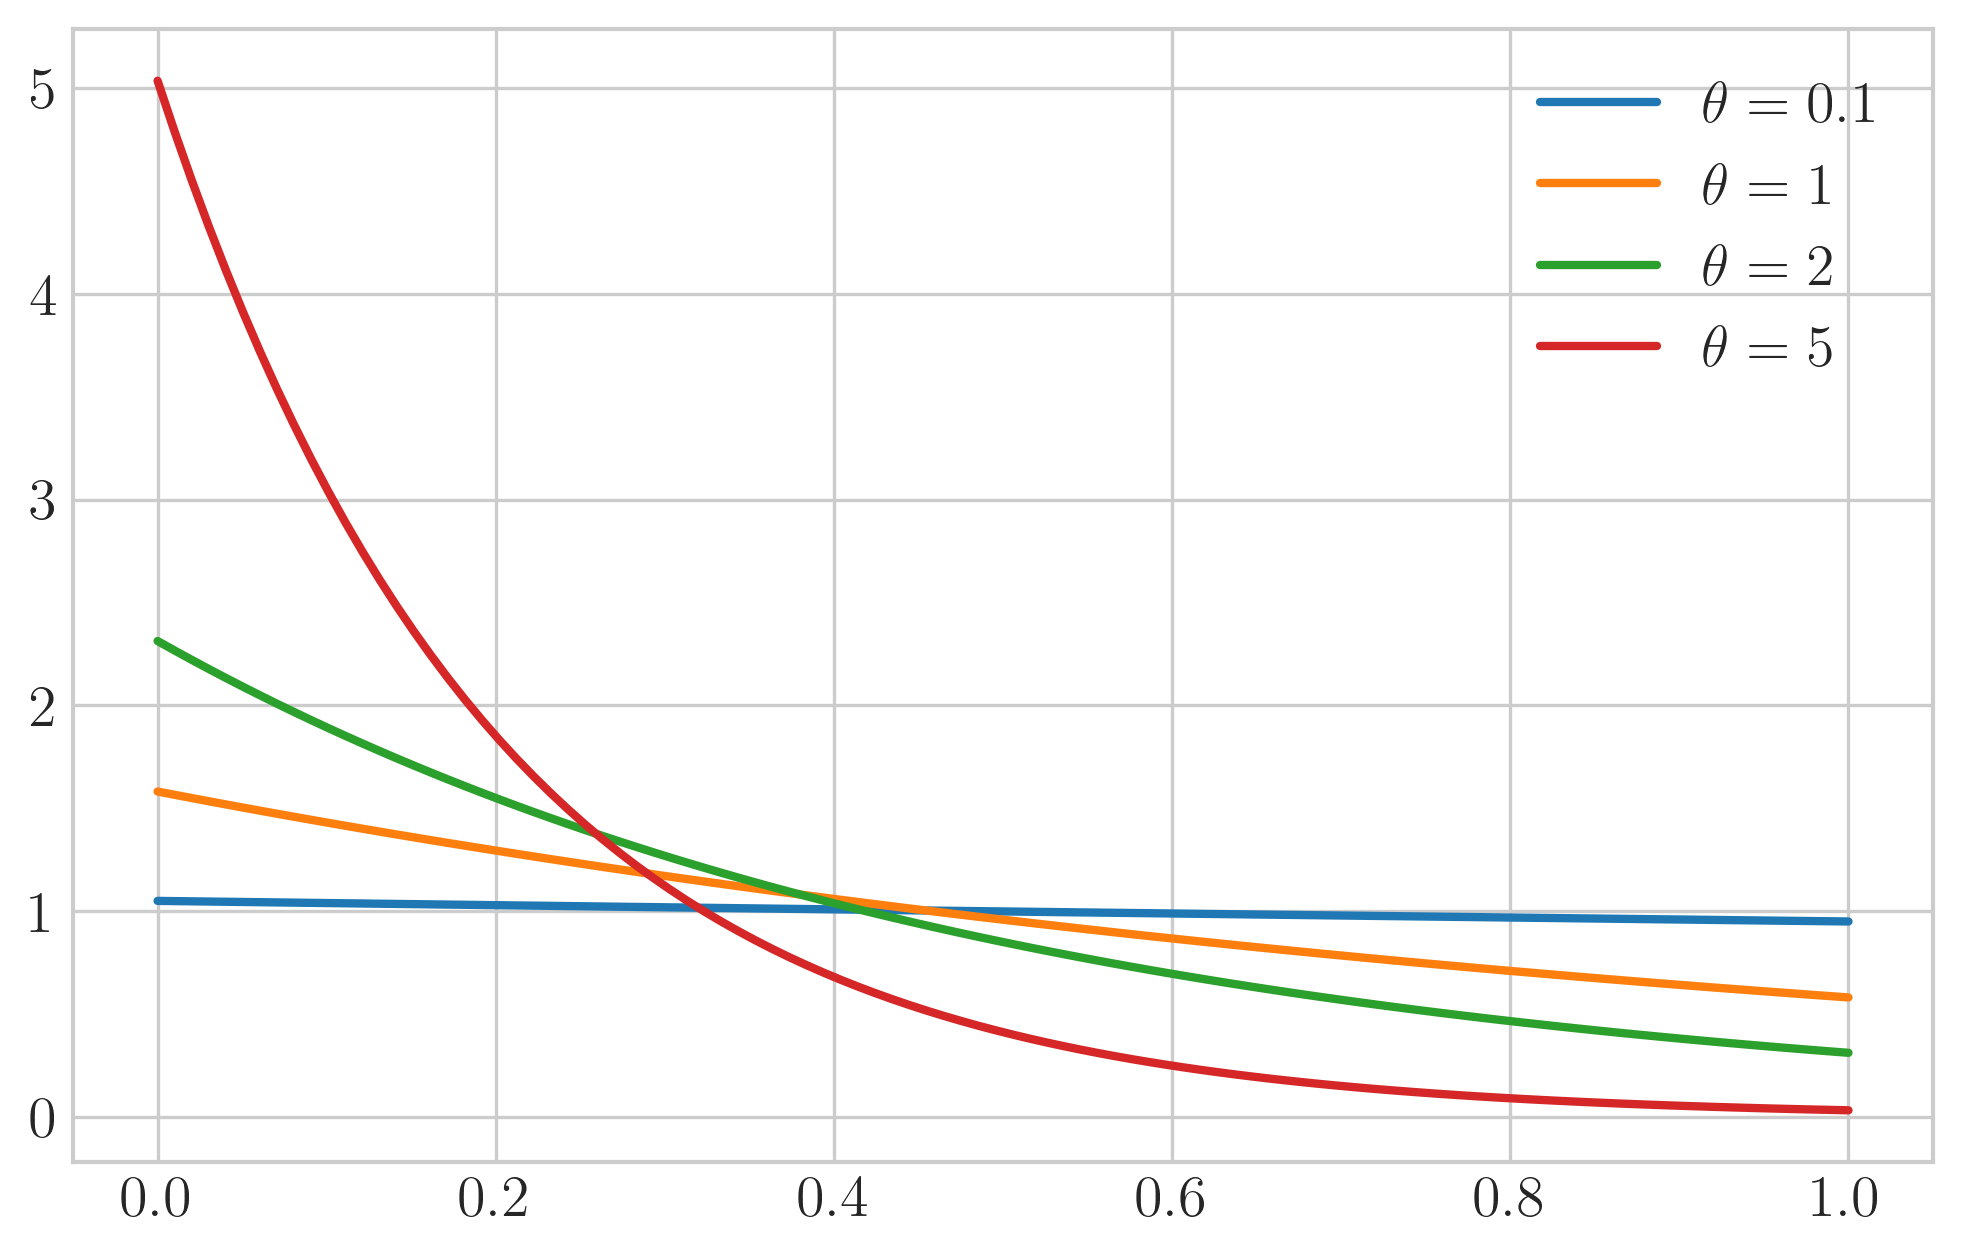
\includegraphics[scale=0.65]{plots/pdf_min_hat.png}
        \caption{Графіки щільності $f_{\widehat{m}}(x)$ для різних значень $\theta$.}
    \end{figure}
    \begin{figure}[H]
        \centering
        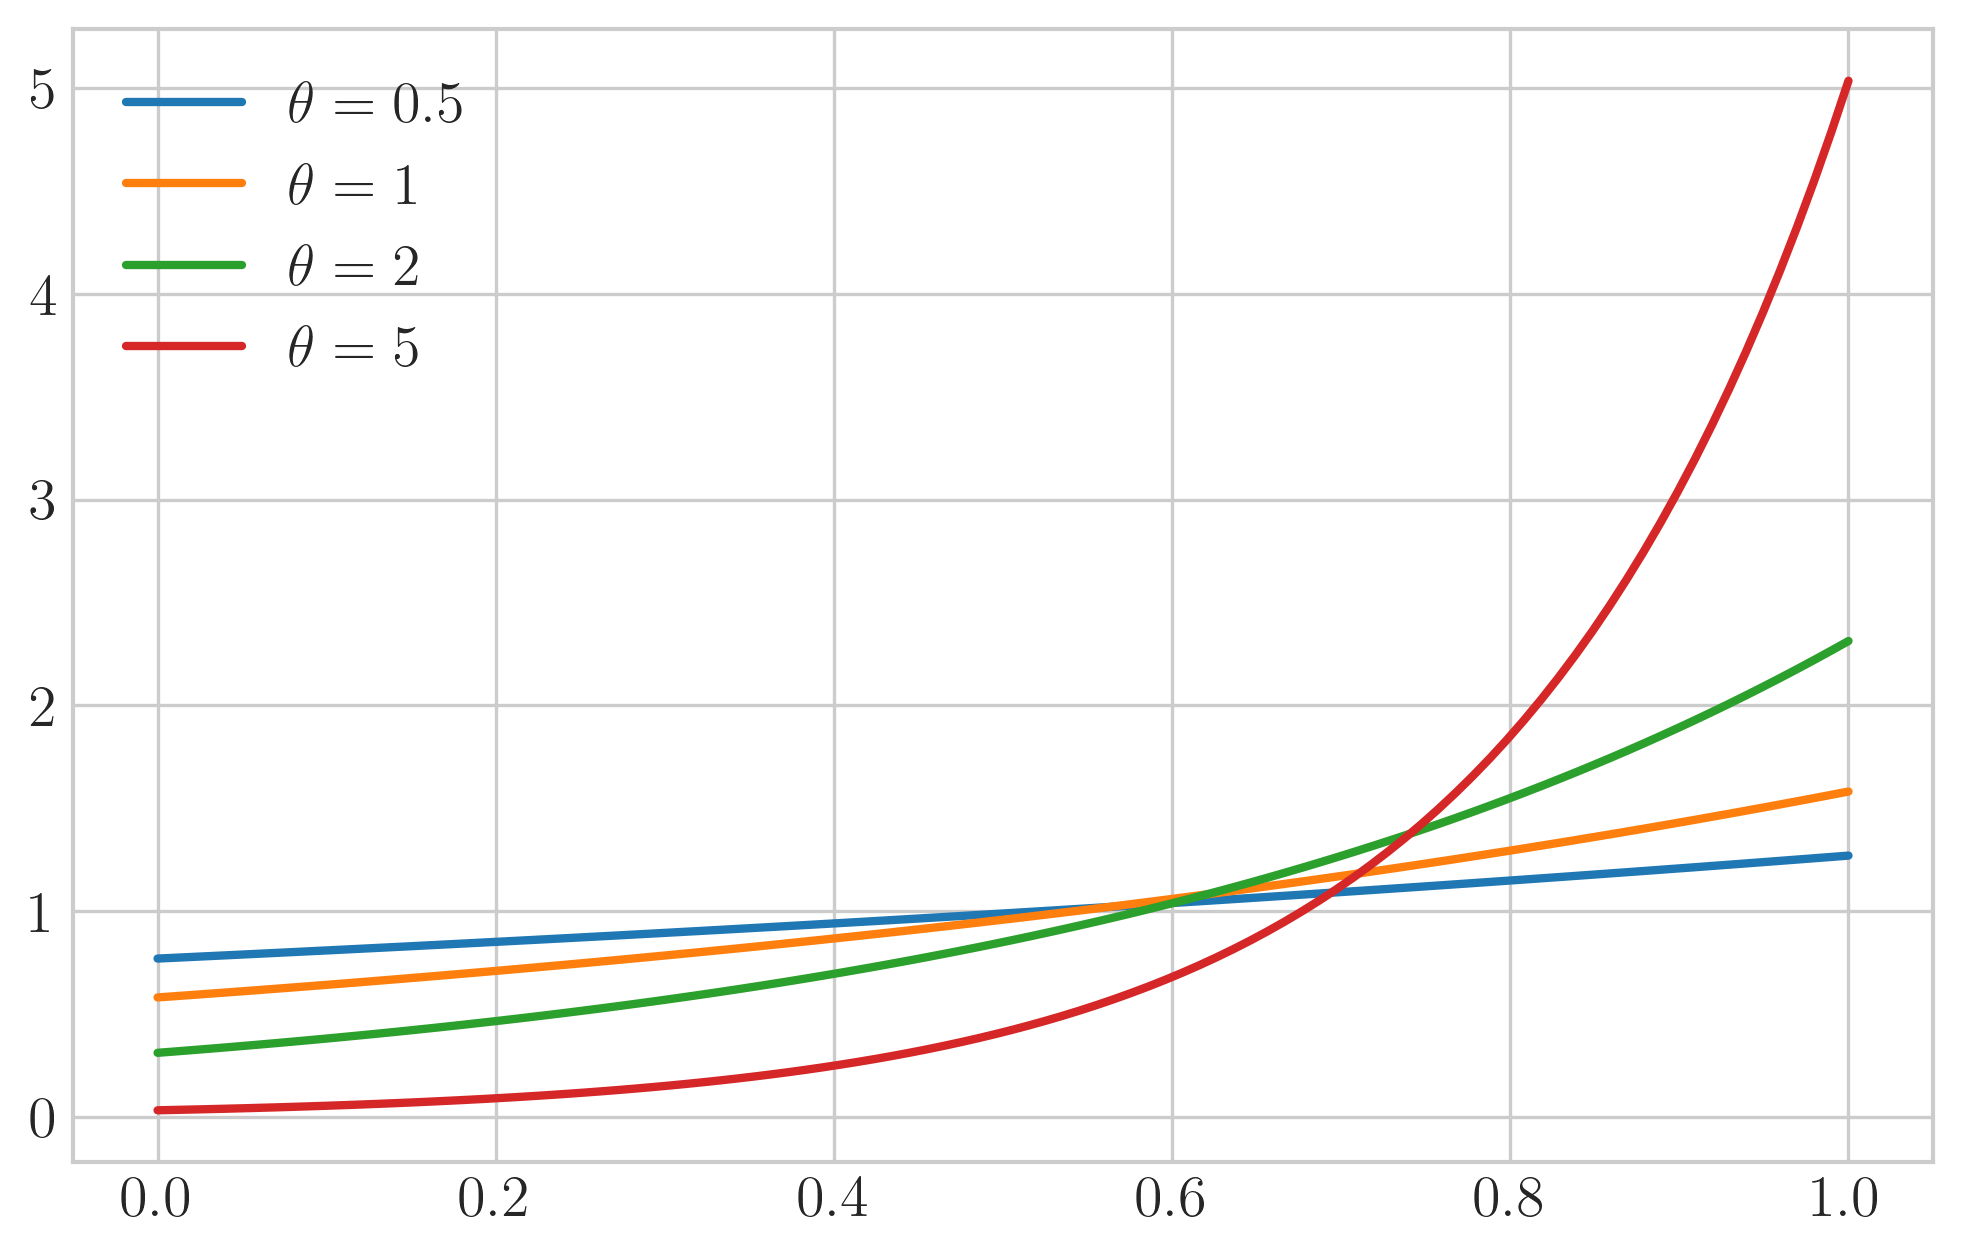
\includegraphics[scale=0.65]{plots/pdf_max_hat.png}
        \caption{Графіки щільності $f_{\widehat{M}}(x)$ для різних значень $\theta$.}
    \end{figure}
\end{theorem}

\subsection{Сума нерухомих точок}
Граничний розподіл суми нерухомих точок можна отримати, користуючись функціоналом Лапласа точкового процесу Пуассона.
Згідно з означенням \ref{def:poiss_proc}, для процесу Пуассона з мірою інтенсивності 
$\theta \cdot \mathrm{Leb}$ на $[0, 1]$ цей функціонал задається як
\begin{equation}\label{laplace_functional}
    \psi_N(f) = \exp\left\{ - \; \theta \int_0^1 \left(1 - e^{-f(x)}\right) \d x\right\}
\end{equation}
для вимірних, невід'ємних, обмежених функцій $f$ на $[0, 1]$.

Позначатимемо $\Sum(N)$ суму атомів точкового процесу Пуассона $N$. 
Для будь-якої точкової міри $\mu$, 
$\Sum(\mu) = \int_0^1 x \d\mu$. 
Перетворення Лапласа невід'ємної випадкової величини $X$ задається
$\L{X}(p) = \E e^{-pX}$. 
Якщо порівняти це означення з \eqref{laplace_functional}, можна побачити, що
перетворення Лапласа $\Sum(N)$ дорівнює значенню $\psi_N(f)$ для $f(x) = px$.
Пряме обчислення дає наступний результат:
\begin{gather}\label{laplace_of_sum}
    \L{\Sum(N)}(p) = 
    \exp\left\{- \theta \left( 1 + \frac{1}{p}(e^{-p} - 1)\right) \right\}.
\end{gather}

Оскільки розподіл $\Sum(N)$ є сумішшю абсолютно неперервного розподілу та
дискретного з атомом в 0, можна знайти перетворення Лапласа
лише абсолютно неперервної частини, що також буде перетворення для
$\Sum(\widehat{N})$.
\begin{gather}
    \L{\Sum(N)}(p) = \E e^{-p\cdot\Sum(N)} = 
    1 \cdot \P{\Sum(N) = 0} + \nonumber \\ +
    \E e^{-p\cdot\Sum(\widehat{N})} \cdot \P{\Sum(N) > 0} =
    e^{-\theta} + \L{\Sum(\widehat{N})}(p) \cdot (1-e^{-\theta})
    \nonumber \\
    \L{\Sum(\widehat{N})}(p) = \frac{1}{1 - e^{-\theta}}
    \left(\L{\Sum(N)}(p) - e^{-\theta}\right) = \nonumber \\ =
    \label{laplace_of_sum_cont}
    \frac{e^{-\theta}}{1 - e^{-\theta}} \cdot 
    \left(\exp\left\{- \frac{\theta}{p}(e^{-p} - 1) \right\} - 1\right)
\end{gather}

$\Sum(\widehat{N})$ є абсолютно неперервною випадковою величиною,
$\L{\Sum(\widehat{N})}(p)$ є перетворенням Лапласа для щільності, тому
перетворення Лапласа для функції розподілу $\Sum(\widehat{N})$
задається 
\begin{equation}\label{sum_cdf_laplace}
    \L{F_{\Sum(\widehat{N})}(x)}(p) = 
    \frac{e^{-\theta}}{1 - e^{-\theta}} \cdot \frac{1}{p} \cdot
    \left(\exp\left\{- \frac{\theta}{p}(e^{-p} - 1) \right\} - 1\right)
\end{equation}
Знаходження оберненого перетворення для \eqref{sum_cdf_laplace}
є доволі складним.

Розглянемо інший підхід до знаходження $F_{\Sum(N)}(x) = \P{\Sum(N) \leq x}$:
\begin{gather*}
    \P{\Sum(N) \leq x} = 
    \sum_{m=0}^{\infty} \P{\Sum(N) \leq x \mid N([0, 1]) = m} \P{N([0, 1]) = m}
    = \\ = \mathds{1}\left\{x\geq 0\right\}\cdot e^{-\theta} +
    \sum_{m=1}^{\infty} \P{\Sum(N) \leq x \mid N([0, 1]) = m} \frac{\theta^m}{m!} e^{-\theta}
\end{gather*}
Згідно з \cite{ContUnivDistr} (ст. 296), умовні розподіли 
$\P{\Sum(N) \leq x \mid N([0, 1]) = m}$
є розподілами Ірвіна-Голла --- розподілами 
суми $m$ незалежних випадкових величин з розподілом $\Unif{0, 1}$. Їх
функція розподілу має вигляд
\begin{gather*}
    F_s^{[m]} (x) = \begin{cases}
        0, & x < 0, \\
        \frac{1}{m!}\sum_{k=0}^{\floor*{x}} (-1)^k C_m^k (x-k)^m, & 0 \leq x < m, \\
        1, & x \geq m.
    \end{cases}
\end{gather*}
Для кожного інтервалу $[n, n+1)$, $n\in \N_0$, 
$\P{\Sum(N) \leq x}$  може бути виражена через $I_{\nu}(z)$, $\nu \in \R$  ---
модифіковані функції Бесселя першого роду (\cite{Abramowitz_Stegun}, ст. 375):
\begin{equation*}
    I_{\nu}(z) = \left(\frac{1}{2} z\right)^{\nu}
    \sum_{k=0}^{\infty} \frac{
        \left(\frac{1}{4} z^2 \right)^{k}
    }{
        k! \Gamma(\nu + k + 1)
    }
\end{equation*}
Отримаємо відповідну формулу. Нехай $x \in [n, n+1)$,
\begin{gather*}
    e^{\theta} \cdot \P{\Sum(N) \leq x} = 
    1 + \sum_{m=1}^{\infty} \P{\Sum(N) \leq x \mid N([0, 1]) = m} \frac{\theta^m}{m!} = \\ =
    1 + \sum_{m=1}^{n} 1 \cdot \frac{\theta^m}{m!} + 
    \sum_{m=n+1}^{\infty} \left(
        \frac{1}{m!}\sum_{k=0}^{n} (-1)^k C_m^k (x-k)^m
    \right) \frac{\theta^m}{m!} = \\ =
    \sum_{m=0}^{n} \frac{\theta^m}{m!} + 
    \sum_{m=n+1}^{\infty} \left(
        \sum_{k=0}^{n} (-1)^k \frac{1}{k! (m-k)!} (x-k)^m
    \right) \frac{\theta^m}{m!} = \\ =
    \sum_{m=0}^{n} \frac{\theta^m}{m!} + 
    \sum_{k=0}^{n} \frac{(-1)^k}{k!} \left(
        \sum_{m=n+1}^{\infty} \frac{1}{m! (m-k)!} (x - k)^m \theta^m
    \right) = \left[m - k = l \right] = \\
    = \sum_{m=0}^{n} \frac{\theta^m}{m!} + 
    \sum_{k=0}^{n} \frac{(-1)^k}{k!} \left(
        \sum_{l=n-k+1}^{\infty} \frac{1}{l! (l+k)!} (x - k)^{l+k} \theta^{l+k}
    \right) = \\ =
    \sum_{m=0}^{n} \frac{\theta^m}{m!} + 
    \sum_{k=0}^{n} \frac{(-1)^k}{k!} (x-k)^k \theta^k
    \left(
        \sum_{l=n-k+1}^{\infty} \frac{1}{l! (l+k)!} (x - k)^{l} \theta^{l}
    \right) = \\ = \left[\frac{1}{l! (l+k)!} (x - k)^{l} \theta^{l} = a_{k, l}\right] = \\ =
    \sum_{m=0}^{n} \frac{\theta^m}{m!} +
    \sum_{k=0}^{n} \frac{(-1)^k}{k!} (x-k)^k \theta^k
    \left(
        \sum_{l=0}^{\infty} a_{k, l} - 
        \sum_{l=0}^{n-k} a_{k, l} 
    \right) = \\
    = \sum_{k=0}^{n} \frac{(-1)^k}{k!}
    \left(\theta (x - k)\right)^{\frac{k}{2}} I_k\left(2\sqrt{\theta(x-k)}\right) + \\ +
    \sum_{m=0}^{n} \frac{\theta^m}{m!}
    - \sum_{k=0}^{n} \sum_{l=0}^{n-k}  \frac{(-1)^k}{k!} \frac{1}{l! (l+k)!} (x - k)^{k+l} \theta^{k+l}
\end{gather*} 
Позначимо $R(n) = \sum_{m=0}^{n} \frac{\theta^m}{m!}$,
$L(n) = \sum_{k=0}^{n} \sum_{l=0}^{n-k} \frac{(-1)^k}{k!} \frac{1}{l! (l+k)!} (x - k)^{k+l} \theta^{k+l}$.
Покажемо, що $R(n) - R(n-1) = L(n) - L(n-1)$ для всіх $n \in \N$:
\begin{gather*}
    R(n) - R(n-1) = \frac{\theta^n}{n!}, \\
    L(n) - L(n-1) = \sum_{k=0}^n \sum_{l=0}^{n-k} s_{k, l} - 
    \sum_{k=0}^{n-1} \sum_{l=0}^{n-k-1} s_{k, l} = \sum_{i=0}^n s_{i, n-i} = \\ =
    \sum_{i=0}^n \frac{(-1)^i}{i!} \frac{1}{(n-i)! n!} (x - i)^n \theta^n = 
    \frac{\theta^n}{n!} \cdot \frac{1}{n!} \sum_{i=0}^n (-1)^i C_n^i (x-i)^n.
\end{gather*}
Розглянемо функцію $f(x) = x^n$.
Ліва скінченна різниця першого порядку для $f$ з кроком $h=1$ --- це 
$\Delta f(x) = f(x) - f(x-1)$, другого порядку --- $\Delta^2 f(x) = \Delta f(x) - \Delta f(x-1) = 
f(x) - 2f(x-1) + f(x-2)$,
аналогічно рекурентно визначаються скінченні різниці вищих порядків.
Загальною формулою для різниці $k$-того порядку буде
$\Delta^k f(x) = \sum_{i=0}^k (-1)^i C_k^i f(x-i) = \sum_{i=0}^k (-1)^i C_k^i (x - i)^n$,
тому вираз $\sum_{i=0}^n (-1)^i C_n^i (x-i)^n$ --- це ліва скінченна різниця $n$-того порядку для
$x^n$. Оскільки кожна скінченна різниця є поліном порядку на 1 менше, ніж попередня,
то різниця $n$-того порядку вже буде константою. Виявляється,
що
\begin{gather*}
    \frac{1}{n!} \Delta^n f(n) = 
    \frac{1}{n!} \sum_{i=0}^n (-1)^i C_n^i (n - i)^n = 
    \frac{1}{n!} \sum_{k=0}^n (-1)^{n-k} C_n^k k^n = {n\brace n} = 1,
\end{gather*}
де ${n \brace m}$ позначає число Стірлінґа другого роду (\cite{Abramowitz_Stegun}, ст. 824-825).
Отже, $R(n) - R(n-1) = L(n) - L(n-1)$ для всіх $n \in \N$. Оскільки
$R(0) = L(0) = 1$, то $R(n) = L(n)$ для всіх $n \in \N$.
Таким чином, отримуємо 
\begin{gather}
    F_{\Sum(N)}(x) = e^{-\theta}
    \sum_{k=0}^{n} \frac{(-1)^k}{k!}
    \left(\theta (x - k)\right)^{\frac{k}{2}} I_k\left(2\sqrt{\theta(x-k)}\right), \; x \in [n, n+1).
\end{gather}
Зауважимо, що 
$F_{\Sum(N)}(0) = \left.e^{-\theta} I_0\left(2 \sqrt{\theta x}\right) \right|_{x = 0} = e^{-\theta} = \P{\Sum(N) = 0}$.

В свою чергу, функція розподілу $\Sum(\widehat{N})$ 
може бути виражена через $F_{\Sum(N)}(x)$ наступним чином:
\begin{gather}
    \P{\Sum(\widehat{N}) \leq x} = \P{\Sum(N) \leq x \mid \Sum(N) > 0} = 
    \begin{cases}
        0, & x < 0, \\
        \frac{F_{\Sum(N)}(x) - e^{-\theta}}{1-e^{-\theta}}, & x \geq 0.
    \end{cases}
\end{gather}
Оскільки $\Sum(\widehat{N})$ є абсолютно неперервною випадковою величиною, можна також знайти
її щільність розподілу. Зробимо це для $x \in [n, n+1), n \in \N_0$. Оскільки
$I_{\nu} ' (z) = I_{\nu+1} (z) + \frac{\nu}{z} I_{\nu} (z)$ (\cite{Abramowitz_Stegun}, ст. 376),
то для $z = z(x) = \sqrt{\theta(x-k)}$ і 
$g_k(x) = g_k(z(x)) = \left(\theta (x - k)\right)^{\frac{k}{2}} I_k\left(2\sqrt{\theta(x-k)}\right) = z^k I_k(2z)$
маємо
\begin{gather*}
    g_k'(x) = \left(
        k z^{k-1} I_k(2z) + 2 z^k \left(I_{k+1}(2z) + \frac{k}{2z} I_k(2z)\right)
    \right) z'(x) = \\ =
    2 z^{k-1} \left(k I_k(2z) + z I_{k+1}(2z)\right) \cdot z'(x) = 
    2 z^{k-1} \left(k I_k(2z) + z I_{k+1}(2z)\right) \cdot \frac{\theta}{2 z} = \\ =
    \theta z^{k-2} \left(k I_k(2z) + z I_{k+1}(2z)\right) = \\ =
    \theta \left(\theta (x - k)\right)^{\frac{k}{2}-1}
    \left(
        k I_k \left(2 \sqrt{\theta (x - k)} \right) + 
        \sqrt{\theta (x - k)} I_{k+1} \left(2 \sqrt{\theta (x - k)}\right)
    \right)
\end{gather*}
Таким чином, отримуємо
\begin{gather}
    f_{\Sum(\widehat{N})}(x) = \frac{e^{-\theta}}{1 - e^{-\theta}} \sum_{k=0}^{n} \frac{(-1)^k}{k!} g_k'(x), \; x \in [n, n+1).
\end{gather}

При цьому, $\E\Sum(N)$ значно простіше знайти
за формулою повного математичного сподівання,
оскільки для $m > 0$ $\E\left(\Sum(N) \mid N([0, 1]) = m\right) = \frac{m}{2}$
як математичне сподівання суми $m$ незалежних випадкових величин
з розподілом $\Unif{0, 1}$:
\begin{gather*}
    \E\Sum(N) = 0\cdot \P{N([0, 1]) = 0} +
    \sum_{m=1}^{\infty} \frac{m}{2} \frac{\theta^m}{m!} e^{-\theta} =
    \frac{e^{-\theta}}{2}\sum_{m=1}^{\infty} \frac{\theta^m}{(m-1)!} = \frac{\theta}{2}
\end{gather*}

Сформулюємо отриманий результат у вигляді теореми.
\begin{theorem}\label{th:sum_limit}
    Нехай $\sigma \sim \ESF{n, \theta}$, а 
    $S_n = \sum_{i : \sigma(i) = i} i = \sum_{i=1}^n i \cdot \mathds{1}\left\{\sigma(i) = i \right\}$ --- сума нерухомих точок $\sigma$.
    Тоді при $n\to\infty$ виконується граничне
    співвідношення
    $\frac{S_n}{n} \overset{d}{\longrightarrow} S$,
    де функція розподілу випадкової величини $S$ дорівнює
    \begin{gather}
        F_{S}(x) = \begin{cases}
            0, & x < 0, \\
            e^{-\theta}
            \sum\limits_{k=0}^{\floor*{x}}
            (-1)^k \frac{1}{k!}\left(\theta(x-k)\right)^{\frac{k}{2}} I_k\left(2\sqrt{\theta(x-k)}\right), & x \geq 0,
        \end{cases}
    \end{gather}
    а її перетворення Лапласа має вигляд \eqref{laplace_of_sum}.
    
    Якщо позначити $\widehat{S}_n$ суму нерухомих точок за умови,
    що вони взагалі існують, то виконуються також граничне співвідношення
    $\frac{\widehat{S}_n}{n} \overset{d}{\longrightarrow} \widehat{S}$,
    де $\widehat{S}$ є абсолютно неперервною випадковою величиною з
    функцією та щільністю розподілу
    \begin{gather}
        F_{\widehat{S}}(x) = \begin{cases}
            0, & x < 0, \\
            \frac{F_{S}(x) - e^{-\theta}}{1 - e^{-\theta}}, & x \geq 0,
        \end{cases},\;
        f_{\widehat{S}}(x) = \begin{cases}
            0, & x < 0, \\
            \frac{\theta e^{-\theta}}{1 - e^{-\theta}}
            \sum_{k=0}^{\floor*{x}} \frac{(-1)^k}{k!} f_k(x), & x \geq 0,
        \end{cases},
    \end{gather}
    де $f_k(x)$ визначено як 
    $$f_k(x) = \left(\theta (x - k)\right)^{\frac{k}{2} - 1}
    \left(
        k I_k \left(2 \sqrt{\theta (x - k)} \right) + 
        \sqrt{\theta (x - k)} I_{k+1} \left(2 \sqrt{\theta (x - k)}\right)
    \right),$$
    а її перетворення Лапласа має вигляд \eqref{laplace_of_sum_cont}.
    \begin{figure}[H]
        \centering
        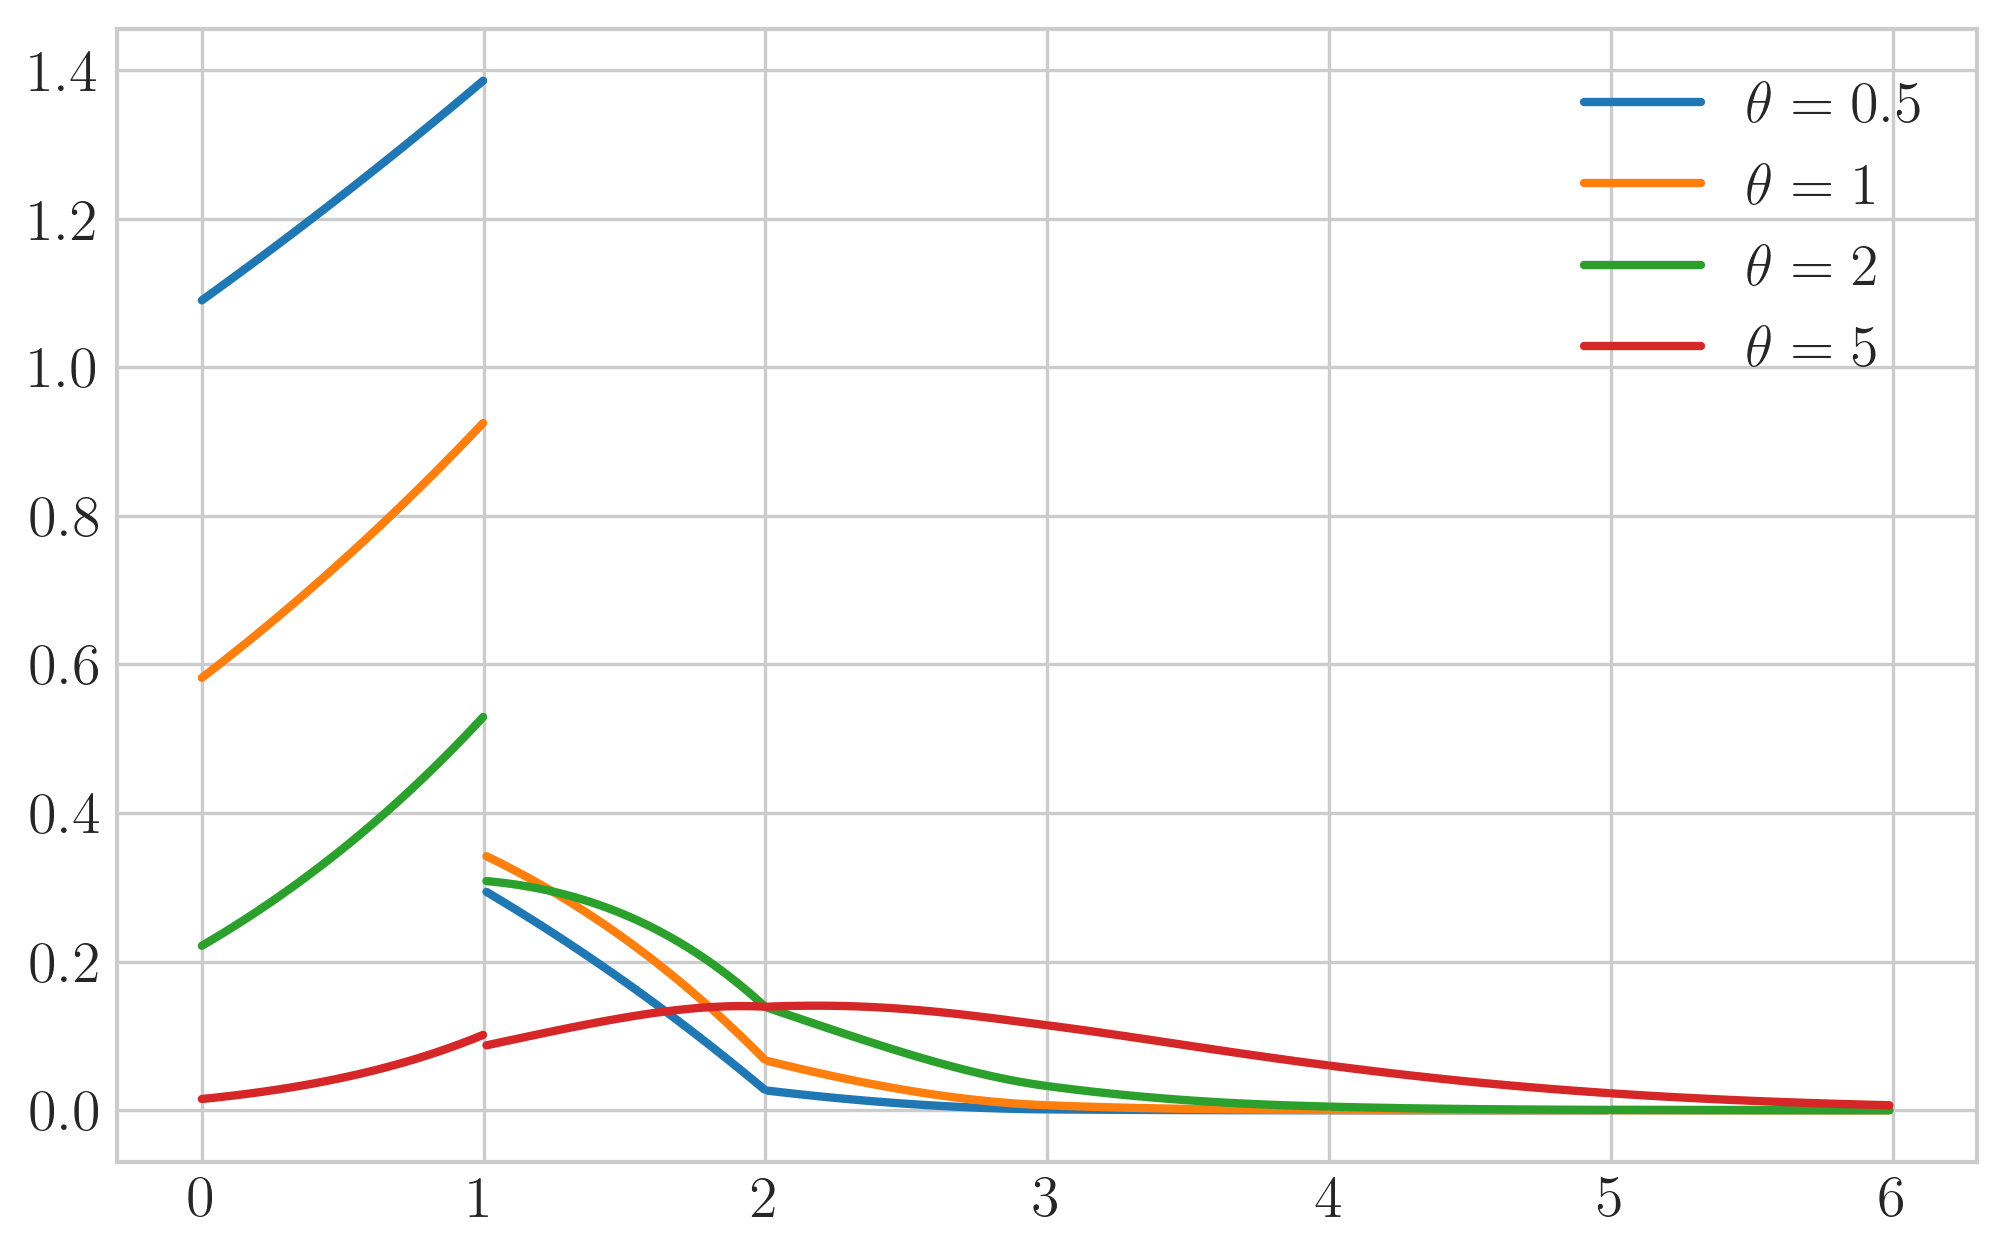
\includegraphics[scale=0.6]{plots/pdf_sum_hat.png}
        \caption{Графіки щільності розподілу $f_{\widehat{S}}(x)$ для різних значень $\theta$.}
    \end{figure}
\end{theorem}

\subsection{Найменший і найбільший спейсинги}
Визначимо граничні розподіли найменшого і найбільшого спейсингів --- відстаней
між сусідніми нерухомими точками.
\begin{remark}
    Щоб застосувати тут теоретичні результати, що стосуються
    випадкового розбиття інтервалів, зручно вважати
    $\min(N)$ і $1-\max(N)$ спейсингами. Для випадкової
    перестановки $\left\{1, \dots, n\right\}$ це означатиме
    вважати $0$ та $n+1$ <<штучними>> нерухомими точками.
\end{remark}

Обґрунтуємо можливість застосування теореми \ref{th:cont_map} до відповідних відображень.
Нехай $\mu$ --- проста точкова міра на $[0, 1]$,
а $\left\{x_1, ..., x_k\right\}$ --- множина її атомів,
які вважатимемо відсортованими, тобто $x_1 < x_2 < ... < x_k$.
Перетворення вектора $\left(x_1, ..., x_k\right)^T$ у вектор
спейсингів $\left(y_1, ..., y_{k+1}\right)$ є лінійним:
\begin{gather*}
    \begin{pmatrix}
        y_1 \\ y_2 \\ y_3 \\ \vdots \\ y_{k-1} \\ y_k \\ y_{k+1}
    \end{pmatrix} = 
    \begin{pmatrix}
        1  & 0  & 0 & \cdots & 0 & 0 \\
        -1 & 1  & 0 & \cdots & 0 & 0 \\
        0  & -1 & 1 & \cdots & 0 & 0 \\
        \vdots & \vdots & \vdots & \ddots& \vdots& \vdots \\
        0  & 0  & 0 & \cdots & 1 & 0 \\
        0  & 0  & 0 & \cdots & -1 & 1 \\
        0  & 0  & 0 & \cdots & 0 & -1
    \end{pmatrix}
    \begin{pmatrix}
        x_1 \\ x_2 \\ x_3 \\ \vdots \\ x_{k-1} \\ x_k
    \end{pmatrix} + 
    \begin{pmatrix}
        0\\ 0 \\ 0 \\ \vdots \\ 0 \\ 0 \\ 1
    \end{pmatrix} = 
    \begin{pmatrix}
        x_1 \\ x_2 - x_1 \\ x_3 - x_2 \\ \vdots \\ x_{k-1} - x_{k-2} \\ x_k - x_{k-1} \\ 1 - x_{k}
    \end{pmatrix}
\end{gather*}
Найменший та найбільший спейсинги
задаються формулами
$\min\left\{y_1,\dots,y_{k+1} \right\}$ та
$\max\left\{y_1,\dots,y_{k+1} \right\}$, відповідно.

Отже, відображення $\smin(\mu)$ та $\smax(\mu)$,
що ставлять у відповідність точковій мірі $\mu$ найменший та найбільший
спейсинги між її атомами, є неперервними функціями
від атомів, тому за теоремою \ref{th:cont_map} є 
неперервними відносно грубої топології.

Як і раніше, розподіли $\smin(N)$ та $\smax(N)$
шукатимемо, користуючись тим, що розподіл атомів $N$ на $[0, 1]$
за умови, що відома їх кількість, є рівномірним.

Нехай $U_1, U_2, \dots, U_{n}$ ---
незалежні випадкові величини
з розподілом $\Unif{0, 1}$, що розділяють відрізок $[0, 1]$ на $n+1$
інтервалів з довжинами $S_1, S_2, \dots, S_{n+1}$, або, у відсортованому вигляді, 
$S_{(1)}^{[n+1]} < S_{(2)}^{[n+1]} < \dots < S_{(n+1)}^{[n+1]}$
(нагадаємо, $S_{(i)}$ позначає $i$-ту порядкову статистику, а
$S_{(i)}^{[n+1]}$ --- те ж саме, але з вказанням $n+1$ як кількості цих статистик).
Розподіли $S_{(k)}^{[n+1]}$ отримано у багатьох роботах
(наприклад, \cite{Holst_1980}, \cite{Pinelis_2019}). Зокрема, для $x\in[0,1]$
\begin{gather}
    \label{min_spacing}
    \P{S_{(1)}^{[n+1]} > x} = \left((1-(n+1)x)_+\right)^n, \\
    \label{max_spacing}
    \P{S_{(n+1)}^{[n+1]} > x} = 
    \sum_{j=1}^{n+1} (-1)^{j-1} C_{n+1}^j \left((1-jx)_+\right)^n,
\end{gather}
де $x_+ = \max(x, 0)$.

Отже, розподіли найменшого $\smin(N)$ та найбільшого $\smax(N)$ спейсингів 
між атомами $N$ задаються
(з домовленістю $S_{(1)}^{[1]} = 1$)
\begin{gather}
    \label{s_min}
    \P{\smin(N) > x} = 
    \sum_{n=0}^{\infty} \P{S_{(1)}^{[n+1]} > x} \P{N([0, 1]) = n}, \\
    \label{s_max}
    \P{\smax(N) > x} = 
    \sum_{n=0}^{\infty} \P{S_{(n+1)}^{[n+1]} > x} \P{N([0, 1]) = n}.
\end{gather}
Хоча явні вирази для \eqref{s_min} та \eqref{s_max},
скоріш за все, доволі складні, цікаво звернути увагу на дві випадкові величини
з такими ж розподілами.

Відомо (наприклад, \cite{Holst_1980}), що для незалежних величин 
$X_1, X_2, \dots, X_{n+1}$ з розподілом $\Exp{1}$
мають місце наступні три рівності:
\begin{gather}
    \label{distr_equal_1}
    \left(
        S_1, S_2, \dots, S_{n+1}
    \right)^T
    \overset{d}{=}
    \left(
        \frac{X_1}{\sum_{i=1}^{n+1} X_i},
        \frac{X_2}{\sum_{i=1}^{n+1} X_i},
        \dots,
        \frac{X_{n+1}}{\sum_{i=1}^{n+1} X_i}
    \right)^T, \\
    \label{distr_equal_2}
    \left(
        S_{(1)}, S_{(2)}, \dots, S_{(n+1)}
    \right)^T
    \overset{d}{=}
    \left(
        \frac{X_{(1)}}{\sum_{i=1}^{n+1} X_i},
        \frac{X_{(2)}}{\sum_{i=1}^{n+1} X_i},
        \dots,
        \frac{X_{(n+1)}}{\sum_{i=1}^{n+1} X_i}
    \right)^T, \\
    \label{distr_equal_3}
    X_{(i)} \overset{d}{=}
    \frac{X_{n+1}}{n+1} + \frac{X_{n}}{n} + \dots + \frac{X_{n-i+2}}{n-i+2} = 
    \sum_{k=0}^{i-1} \frac{X_{n+1-k}}{n+1-k}.
\end{gather}
Рівності \eqref{distr_equal_2} та \eqref{distr_equal_3}
можна доповнити наступною рівністю:
\begin{lemma}\label{distr_equal}
    Для порядкових статистик спейсингів 
    $S_{(1)}^{[n+1]}, ..., S_{(n+1)}^{[n+1]}$
    між незалежними величинами з розподілом $\Unif{0, 1}$
    та незалежних величин 
    $X_1, X_2, \dots, X_{n+1}$ з розподілом $\Exp{1}$ має місце
    рівність 
    \begin{gather}\label{distr_equal_4}
        S_{(i)}^{[n+1]} \overset{d}{=}
        \frac{
            \frac{X_{n+1}}{n+1} + \frac{X_{n}}{n} + \dots + \frac{X_{n-i+2}}{n-i+2}
        }{
            \sum_{j=1}^{n+1} X_j
        } = \frac{
            \sum_{k=0}^{i-1} \frac{X_{n+1-k}}{n+1-k}
        }{
            \sum_{j=1}^{n+1} X_j
        }, \; i = 1, \dots, n+1.
    \end{gather}
\end{lemma}
\begin{proof}
    Позначимо спейсинги між $X_1, X_2, \dots, X_{n+1}$ через
    $\Delta_1 = X_{(1)}$,
    $\Delta_i = X_{(i)} - X_{(i-1)}, i=2, \dots, n+1$. З \cite{Arnold_et_al_2008}, ст. 72, відомо, що
    всі $\Delta_i$ незалежні та мають розподіли $\Exp{n-i+2}$.
    Отже, праву частину $S_{(i)} \overset{d}{=} \frac{X_{(i)}}{\sum_{j=1}^{n+1}X_j}$
    можна переписати як
    \begin{gather*}
        \frac{X_{(i)}}{\sum_{j=1}^{n+1}X_j} = 
        \frac{X_{(i)}}{\sum_{j=1}^{n+1}X_{(j)}} = 
        \frac{
            \Delta_1 + \dots + \Delta_i
        }{
            \Delta_1 + \left(\Delta_1 + \Delta_2\right) +
            \dots + \left(\Delta_1 + \dots + \Delta_{n+1}\right)
        }.
    \end{gather*}
    Введемо нові незалежні випадкові величини
    $Y_i = (n-i+2)\Delta_i$ з розподілом
    $\Exp{1}$. В термінах $Y_i$
    верхню рівність можна переписати як
    \begin{gather*}
        \frac{X_{(i)}}{\sum_{j=1}^{n+1}X_j} = 
        \frac{
            \sum_{j=1}^i \frac{Y_j}{n-j+2} 
        }{
            \sum_{j=1}^{n+1} Y_j
        }.
    \end{gather*}
    Оскільки $X_i$ та $Y_i$ незалежні та мають однакові розподіли, то отримуємо \eqref{distr_equal_4}.
\end{proof}

Окремими випадками леми \ref{distr_equal}
є рівності для мінімального і максимального спейсингів
$S_{(1)}^{[n+1]} \overset{d}{=} \frac{X_{n+1}}{(n+1)\sum_{i=1}^{n+1} X_i}$
та $S_{(n+1)}^{[n+1]} \overset{d}{=} \frac{\sum_{i=1}^{n+1} \frac{X_i}{n-i+2}}{\sum_{i=1}^{n+1} X_i}
\overset{d}{=} \frac{\sum_{i=1}^{n+1} \frac{X_i}{i}}{\sum_{i=1}^{n+1} X_i}$.
Разом з \eqref{s_min} та \eqref{s_max}
вони приводять до наступних рівностей за розподілом:
\begin{gather}\label{distr_equal_5}
    \smin(N) \overset{d}{=}
    \frac{X_{\nu+1}}{(\nu+1)\sum_{i=1}^{\nu+1} X_i} , \;
    \smax(N) \overset{d}{=} 
    \frac{\sum_{i=1}^{\nu+1} \frac{X_i}{i}}{\sum_{i=1}^{\nu+1} X_i},
\end{gather}
де $\nu$ має розподіл $\Poiss{\theta}$, а $\left(X_i, i\geq 1\right)$ незалежні між собою та від $\nu$ 
і мають розподіл $\Exp{1}$.

Відповідні математичні сподівання $\E\smin(N)$ та $\E\smax(N)$ можна знайти з \eqref{distr_equal_5}. 
Нехай $n \in \N_0$, тоді
\begin{gather*}
    \E\left(
        \frac{X_{n+1}}{(n+1)\sum_{i=1}^{n+1} X_i}
    \right) = \frac{1}{(n+1)^2}\cdot \E \left(
        \frac{X_1}{\sum_{i=1}^{n+1} X_i} + \dots + \frac{X_{n+1}}{\sum_{i=1}^{n+1} X_i}
    \right) = \frac{1}{(n+1)^2}, \\
    \E\left(
        \frac{\sum_{i=1}^{n+1} \frac{X_i}{i}}{\sum_{i=1}^{n+1} X_i}
    \right) = 
    \sum_{i=1}^{n+1} \frac{1}{i} \cdot \E\left(\frac{X_i}{\sum_{i=1}^{n+1} X_i}\right) = 
    \frac{1}{n+1} \cdot \sum_{i=1}^{n+1} \frac{1}{i}.
\end{gather*}
Оскільки $\P{\nu = n} = \frac{\theta^n}{n!}e^{-\theta}$, то
\begin{gather*}
    \E\smin(N) = \frac{e^{-\theta}}{\theta}\sum_{n=1}^{\infty} \frac{\theta^n}{n\cdot n!} =
    \frac{e^{-\theta}}{\theta} \sum_{n=1}^{\infty} \frac{1}{n!} \int_0^{\theta} t^{n-1} \d t = 
    \frac{e^{-\theta}}{\theta} \int_0^{\theta} \left( \sum_{n=1}^{\infty} \frac{t^{n-1}}{n!} \right) \d t = \\ =
    \frac{e^{-\theta}}{\theta} \int_0^{\theta} \frac{1}{t} \left( \sum_{n=1}^{\infty} \frac{t^{n}}{n!} \right) \d t = 
    \frac{e^{-\theta}}{\theta}\int_0^\theta \frac{e^t-1}{t}\d t, \\
    \E\smax(N) = \frac{e^{-\theta}}{\theta}\sum_{n=1}^{\infty} \frac{H_n}{n!} \theta^n = 
    \frac{e^{-\theta}}{\theta}\sum_{n=1}^{\infty} \frac{\theta^n}{n!} \int_0^1 \left(1 + s + ... + s^{n-1}\right) \d s = \\ =
    \frac{e^{-\theta}}{\theta}\sum_{n=1}^{\infty} \frac{\theta^n}{n!} \int_0^1 \frac{1 - s^n}{1 - s} \d s = 
    \frac{e^{-\theta}}{\theta} \int_0^1 \frac{1}{1 - s} \left(
        \sum_{n=1}^{\infty} \frac{(1 - s^n)\theta^n}{n!}
    \right) \d s = \\ =
    \frac{e^{-\theta}}{\theta} \int_0^1 \frac{e^{\theta} - e^{s \theta}}{1 - s} \d s = 
    \left[ t = \theta (1 - s)\right] = 
    \frac{e^{-\theta}}{\theta} \int_0^{\theta} \frac{e^{\theta} - e^{\theta - t}}{t} \d t = 
    \frac{1}{\theta} \int_0^{\theta} \frac{1-e^{-t}}{t}\d t.
\end{gather*}
де $H_n = \sum_{k=1}^n \frac{1}{k}$ --- $n$-те гармонічне число.
Зокрема, для $\theta = 1$ (випадок рівномірного розподілу) 
$\E\smin(N) \approx 0.48483$ і $\E\smax(N) \approx 0.7966$.

Сформулюємо отриманий результат у вигляді теореми.
\begin{theorem}\label{th:spacing_limit}
    Нехай $\sigma \sim \ESF{n, \theta}$, а $\delta_n$ та $\Delta_n$ ---
    відповідно, найменша та найбільша відстані між нерухомими точками $\sigma$.
    Тоді при $n\to\infty$ виконуються граничні
    співвідношення
    $\frac{\delta_n}{n} \overset{d}{\longrightarrow} \delta$ і 
    $\frac{\Delta_n}{n} \overset{d}{\longrightarrow} \Delta$, де
    \begin{gather}
        \delta \overset{d}{=}
        \frac{X_{\nu+1}}{(\nu+1)\sum_{i=1}^{\nu+1} X_i}, \;
        \Delta \overset{d}{=} 
        \frac{\sum_{i=1}^{\nu+1} \frac{X_i}{i}}{\sum_{i=1}^{\nu+1} X_i},
    \end{gather}
    для незалежних між собою $\left(X_i, i \geq 1\right)$
    з розподілом $\Exp{1}$ та $\nu \sim \Poiss{\theta}$,
    незалежної від $\left(X_i, i \geq 1\right)$.
\end{theorem}
    \likesection{Висновки}
        % !TEX root = ../main.tex
В цьому розділі було доведено низку теорем,
що стосуються граничної поведінки нерухомих точок
випадкової перестановки $\sigma \sim \ESF{n, \theta}$
при $n \to \infty$. Головним результатом є 
доведення грубої збіжності за розподілом 
послідовності точкових процесів, визначених
\eqref{Pn_def}, яка дозволяє досліджувати
розміщення нерухомих точок. Так, застосування
теореми про неперервне відображення \ref{th:cont_map}
дає можливість дослідити граничні розподіли будь-яких
випадкових величин, пов'язаних з нерухомими точками, 
які можна записати як
неперервні функції від декількох дійсних змінних 
(хоча б на одиничному кубі).
Як приклад, було розглянуто розподіли найменшої та найбільшої
нерухомих точок, суми нерухомих точок, найменшого та найбільшого
спейсингів між ними.
\chapter{Чисельне моделювання та дослідження збіжності}
    \section{Алгоритми для генерування перестановок}
        % !TEX root = ../main.tex
Для чисельних перевірок доведених граничних теорем та демонстрації збіжності
необхідно користуватися якимось алгоритмом для отримання вибірок
з розподілу \eqref{ESF}. 
У \cite{Arratia} наводиться два підходи,
засновані на понятті каплінгу: побудові такого випадкового вектора
$\left(X_1, ..., X_n\right)^T$ зі значенням в
$\left\{1,...,n\right\}^n$, координати якого певним чином
будуть утворювати незалежні цикли, з яких утвориться перестановка
з потрібним розподілом (нагадаємо, в силу теореми \ref{th:perm_decomposition}
кожна перестановка однозначно представляється композицією циклів
з точністю до їх порядку). 

\subsection{Процес китайського ресторану}
Розглянемо випадкові величини $A_1, A_2, ...$ з розподілами
\begin{gather}\label{chinese_rest}
    \P{A_i = j} = \begin{cases}
        \frac{\theta}{\theta + i - 1}, & j = i, \\
        \frac{1}{\theta + i - 1}, & j = 1, 2, ..., i-1.
    \end{cases}
\end{gather}
Перший незалежний цикл починається з 1. 2 додається до цього циклу справа
(і він стає циклом $(1, 2)$) з ймовірністю $\frac{1}{\theta+1}$,
або ж починає новий цикл з ймовірністю $\frac{\theta}{\theta+1}$.
Нехай перші $k-1$ натуральних чисел вже розставлені в цикли.
Тоді $k$ або починає новий цикл з ймовірністю $\P{A_k = k} = \frac{\theta}{\theta + k - 1}$,
або додається справа від $j$ у вже наявний цикл з ймовірністю
$\P{A_k = j} = \frac{1}{\theta + k - 1}$, $j = 1,...,k-1$.
З алгоритму побудови отримуємо, що ймовірність отримати перестановку
на $\left\{1,...,n\right\}$
з $k$ циклами дорівнює
$\frac{\theta^{k-1}}{
    (\theta + 1) \dots (\theta + n - 1)
} = 
\frac{\theta^{k}}{
    \theta(\theta + 1) \dots (\theta + n - 1)
}
$, як і в формулі \eqref{ESF}.

Цикли, отримані за цим алгоритмом, впорядковані наступним чином:
перший містить 1, другий --- найменше число, яке не ввійшло в перший, і так далі.

Варто також зауважити, що цей алгоритм дозволяє отримати не просто
випадкову перестановку з розподілом $\ESF{n, \theta}$,
а послідовність перестановок з розподілами 
$\ESF{2, \theta}, ..., \ESF{n-1, \theta}$, причому два числа,
що в якийсь момент опинилися в одному циклі, завжди залишаються в ньому ж.

Розглянемо приклад для $n = 3$, який можна проілюструвати наступною діаграмою:
\begin{center}
    \begin{tikzpicture}[auto,vertex/.style={draw,ellipse,minimum width=60pt}]
        \node[vertex] (one) {$(1)$};
        \node[vertex, above right=1.5cm and 2.5cm of one] (onetwo) {$(1, 2)$};
        \node[vertex, below right=1.5cm and 2.5cm of one] (one_two) {$(1) (2)$};
        \node[vertex, right=5cm of onetwo] (onetwothree) {$(1, 2, 3)$};
        \node[vertex, below right=0.75 and 5cm of onetwo] (onetwo_three) {$(1, 2) (3)$};
        \node[vertex, above right=0.75cm and 3cm of onetwo] (onethreetwo) {$(1, 3, 2)$};
        \node[vertex, above right=0.75cm and 3cm of one_two] (onethree_two) {$(1, 3) (2)$};
        \node[vertex, right=5cm of one_two] (one_twothree) {$(1) (2, 3)$};
        \node[vertex, below right=0.75cm and 2.5cm of one_two] (one_two_three) {$(1) (2) (3)$};
        \path[-{Stealth[]}, every node/.style={sloped,anchor=south,auto=false}]
            % (one) edge node {$\frac{1}{\theta + 1}$} (onetwo)
            % (one) edge node[below] {$\frac{\theta}{\theta + 1}$} (one_two)
            % (onetwo) edge node {$\frac{1}{\theta + 2}$} (onetwothree)
            % (onetwo) edge node {$\frac{1}{\theta + 2}$} (onethreetwo)
            % (onetwo) edge node[below] {$\frac{\theta}{\theta + 2}$} (onetwo_three)
            % (one_two) edge node {$\frac{1}{\theta + 2}$} (onethree_two)
            % (one_two) edge node {$\frac{1}{\theta + 2}$} (one_twothree)
            % (one_two) edge node[below] {$\frac{\theta}{\theta + 2}$} (one_two_three);
            (one) edge node {$A_2 = 1$} (onetwo)
            (one) edge node[below] {$A_2 = 2$} (one_two)
            (onetwo) edge node {$A_3 = 2$} (onetwothree)
            (onetwo) edge node {$A_3 = 1$} (onethreetwo)
            (onetwo) edge node[below] {$A_3 = 3$} (onetwo_three)
            (one_two) edge node {$A_3 = 1$} (onethree_two)
            (one_two) edge node {$A_3 = 2$} (one_twothree)
            (one_two) edge node[below] {$A_3 = 3$} (one_two_three);
    \end{tikzpicture}
\end{center}
З цієї діаграми видно, що ймовірність отримати перестановку $(1) (2, 3)$
обчислюється як 
$\P{A_3 = 2} \cdot \P{A_2 = 1} = \frac{1}{\theta + 2} \cdot \frac{\theta}{\theta + 1}$.
Аналогічно можна перевірити, шо ймовірність отримати інші перестановки з двома циклами
теж дорівнює $\frac{1}{\theta + 2} \cdot \frac{\theta}{\theta + 1}$,
перестановку $(1, 2, 3)$ з одним циклом --- $\frac{1}{\theta + 2} \cdot \frac{1}{\theta + 1}$,
а тотожну перестановку $(1)(2)(3)$ з трьома циклами ---
$\frac{\theta}{\theta + 2} \cdot \frac{\theta}{\theta + 1}$.

\subsection{Каплінг Феллера}
Розглянемо  незалежні випадкові величини
$B_1, B_2, ...$ з розподілами
\begin{gather}
    \P{B_i = j} = \begin{cases}
        \frac{\theta}{\theta + i - 1}, & j = 1, \\
        \frac{i - 1}{\theta + i - 1}, & j = 0.
    \end{cases}
\end{gather}
Знову почнемо перший незалежний цикл з 1. Якщо $B_n = 1$,
то цей цикл закінчується, а новий починається з 2, а інакше ---
довільно (з рівними ймовірностями) обирається число одне з $n-1$ чисел,
що залишились, і додається до цього циклу справа від 1.
На наступному кроці, якщо $B_{n-1} = 1$, то поточний цикл
закінчується, а новий починається з найменшого
натурального числа, що ще не потрапило до циклів, а інакше ---
довільно обирається одне з $n-2$ чисел і додається до поточного циклу справа.
Цей процес повторюється, доки не утвориться перестановка,
що буде реалізацією $\ESF{n, \theta}$.

Якщо порівнювати цей каплінг з процесом китайського ресторану,
то можна помітити, що $B_i = \mathds{1}\left\{A_i = 1\right\}$, де
$A_i$ визначено \eqref{chinese_rest}. Різницею є те, що
каплінг Феллера використовує $A_1,...,A_n$ в зворотному порядку, 
а отже --- за допомогою нього можна отримувати 
перестановки лише для наперед заданого $n$. Зауважимо, що кількість
циклів у отриманій перестановці рівна $\sum_{i=1}^n B_i$. 

Розглянемо приклад для $n = 5$. Нехай реалізацією величин $(B_1, B_2, B_3, B_4, B_5)$ є
$(0, 1, 1, 0, 0)$. $B_5 = 0$, тому до першого циклу $(1)$ додається довільно вибране
число з $\left\{2,3,4,5\right\}$ --- наприклад, $3$. Оскільки $B_4 = 0$, то до циклу
$(1, 3)$ додається довільно вибране число з $\left\{2, 4, 5\right\}$ --- наприклад, 4.
Оскільки $B_3 = 1$, то поточний цикл $(1, 3, 4)$ закінчується, а наступний починається з 2.
Нарешті, оскільки $B_2 = 1$, то 5 утворює новий цикл, і отримуємо
перестановку $(1, 3, 4) (2) (5)$.
    \section{Перевірка отриманих результатів}
        % !TEX root = ../main.tex
Для перевірки результатів леми \ref{main_lemma} та теорем
\ref{th:min_max_limit}, \ref{th:sum_limit}, \ref{th:spacing_limit}
скористаємося процесом китайського ресторану для отримання вибірок
з $\ESF{n, \theta}$. Розмір вибірки $m$ в усіх випадках буде рівний 3000.

\subsection{Розподіл кількості нерухомих точок}
Для демонстрації збіжностей
$\P{X_n = k} \to \P{X = k}$, де $X \sim \Poiss{\theta}$,
а $X_n$ визначено в лемі \ref{main_lemma} при $\gamma = 1$,
порівняємо полігони розподілу для $X_n$ при $n = 50, 100, 500$ для
різних значень $\theta$. Ймовірності $\P{X_n = k}$ отримуватимемо наближено
за допомогою закону великих чисел: 
\begin{gather*}
    \P{X_n = k} \approx \frac{1}{m} \sum_{i=1}^m \mathds{1}\left\{ 
        \card\left\{j\in \left\{1,\dots,n\right\} : \sigma_i(j) = j\right\} = k
    \right\},
\end{gather*}
де $\sigma_i \sim \ESF{n, \theta}$ і незалежні.

\makeatletter
    \@for\t:={0.5,1,2,5}\do{
        \begin{figure}[H]
            \centering
            \includegraphics[scale=0.6]{plots/fp_prob_theta_\t.png}
            \caption{Полігони розподілу $X_n$ та $X$ для $\theta = \t$.}
        \end{figure}
    }
\makeatother

Видно, що збіжність ймовірностей дійсно присутня, але для більших
значень $\theta$ вона є повільнішою.

\subsection{Розподіл найменшої та найбільшої нерухомих точок}
Для демонстрації збіжностей
$\frac{\widehat{m}_n}{n} \overset{d}{\longrightarrow} \widehat{m}$ і
$\frac{\widehat{M}_n}{n} \overset{d}{\longrightarrow} \widehat{M}$,
доведених в теоремі \ref{th:min_max_limit}, порівняємо
гістограми $\frac{\widehat{m}_n}{n}$ та $\frac{\widehat{M}_n}{n}$
для $n = 500$ з щільностями розподілу $\widehat{m}$ та $\widehat{M}$
для різних значень $\theta$.

\makeatletter
    \@for\t:={0.5,1,2,5}\do{
        \begin{figure}[H]
            \centering
            \includegraphics[scale=0.6]{plots/fp_min_theta_\t.png}
            \caption{Гістограма $\frac{\widehat{m}_n}{n}$ та щільність $\widehat{m}$ для $\theta = \t$.}
        \end{figure}
    }
\makeatother

\makeatletter
    \@for\t:={0.5,1,2,5}\do{
        \begin{figure}[H]
            \centering
            \includegraphics[scale=0.6]{plots/fp_max_theta_\t.png}
            \caption{Гістограма $\frac{\widehat{M}_n}{n}$ та щільність $\widehat{M}$ для $\theta = \t$.}
        \end{figure}
    }
\makeatother

\subsection{Розподіл суми нерухомих точок}
Для демонстрації збіжності
$\frac{\widehat{S}_n}{n} \overset{d}{\longrightarrow} \widehat{S}$
доведеної в теоремі \ref{th:sum_limit}, порівняємо
гістограми $\frac{\widehat{S}_n}{n}$
для $n = 500$ з щільностями розподілу $\widehat{S}$
для різних значень $\theta$.

\makeatletter
    \@for\t:={0.5,1,2,5}\do{
        \begin{figure}[H]
            \centering
            \includegraphics[scale=0.6]{plots/fp_sum_theta_\t.png}
            \caption{Гістограма $\frac{\widehat{S}_n}{n}$ та щільність $\widehat{S}$ для $\theta = \t$.}
        \end{figure}
    }
\makeatother

\subsection{Розподіл найменшого і найбільшого спейсингів}
Для демонстрації збіжностей
$\frac{\delta_n}{n} \overset{d}{\longrightarrow} \delta$ і
$\frac{\Delta_n}{n} \overset{d}{\longrightarrow} \Delta$,
доведених в теоремі \ref{th:spacing_limit}, порівняємо
емпіричні функції розподілу $\frac{\delta_n}{n}$ та $\frac{\Delta_n}{n}$
при $n = 50, 100, 500$ з емпіричними функціями $\delta$ та $\Delta$
для різних значень $\theta$.

Емпіричну функцію розподілу випадкової величини $X$ за вибіркою
$X_1, ..., X_N$ тут визначено як 
$F^*_X(x) = \frac{1}{m} \sum_{i=0}^{m} \mathds{1}\left\{X_i \leq x\right\}$.

Оскільки для $x \geq 1$ 
$\P{\frac{\delta_n}{n} \leq x} = \P{\frac{\Delta_n}{n} \leq x} = \P{\delta \leq x} = \P{\delta \leq x} = 1$,
то на всіх рисунках емпіричні функції розподілу зображено лише для $x \in [0, 1)$.

\makeatletter
    \@for\t:={0.5,1,2,5}\do{
        \begin{figure}[H]
            \centering
            \includegraphics[scale=0.6]{plots/fp_spacing_min_theta_\t.png}
            \caption{Емпіричні функції розподілу $\frac{\delta_n}{n}$ та $\delta$ для $\theta = \t$.}
        \end{figure}
    }
\makeatother

\makeatletter
    \@for\t:={0.5,1,2,5}\do{
        \begin{figure}[H]
            \centering
            \includegraphics[scale=0.6]{plots/fp_spacing_max_theta_\t.png}
            \caption{Емпіричні функції розподілу $\frac{\Delta_n}{n}$ та $\Delta$ для $\theta = \t$.}
        \end{figure}
    }
\makeatother
    \likesection{Висновки}
        % !TEX root = ../main.tex
В цьому розділі було розглянуто алгоритми
для отримання перестановок Юенса, за допомогою
яких було перевірено твердження доведених граничних теорем.
Варто зазначити, що обидва алгоритми є досить
повільними для отримання вибірок великого розміру
для великих значень $n$, оскільки кожна перестановка генерується
послідовно. Натомість, наближені значення потрібної
статистики можна отримувати дуже швидко, якщо для неї
доведено граничну теорему і отримано явний вигляд
граничного розподілу.
\likechapter{Висновки}
    % !TEX root = ../main.tex
\hspace{\parindent}
В даній дипломній роботі було розглянуто випадкові перестановки Юенса
$\sigma \sim \ESF{n, \theta}$, задані розподілом \eqref{ESF}. 
Через нерухомі точки таких перестановок означено послідовність 
точкових процесів $P_n$ на $[0, 1]$ формулою
\eqref{Pn_def} та доведено збіжність при $n \to \infty$ цієї
послідовності до однорідного точкового процесу
Пуассона з інтенсивністю $\theta$ в двох,
в цьому випадку еквівалентних, сенсах --- грубу
збіжність за розподілом та збіжність в топології Скорохода.

За допомогою теореми про неперервне відображення
\ref{th:cont_map} було доведено граничні теореми для
деяких статистик, пов'язаних з нерухомими точками
перестановок Юенса, а саме --- найменшої та найбільшої точок, 
суми точок і найменшої та найбільшої
відстаней між сусідніми нерухомими точками (спейсингів).
Для відповідних граничних випадкових величин було отримано
розподіли в явному вигляді. Усі ці величини є змішаними, 
оскільки з ненульовою ймовірністю
нерухомих точок може не бути взагалі, тому розглянуто
також їх абсолютно неперервні версії, розподіли яких отримані 
накладанням умови існування таких точок.

Результат теореми \ref{main_th} є найважливішим у роботі,
оскільки в поєднанні з теоремою \ref{th:cont_map} дозволяє 
отримувати граничні теореми для всіх статистик, які можна представити
як неперервні функції від атомів точкової міри. Однак він не є вичерпним
з точки зору дослідження властивостей перестановок Юенса,
оскільки стосується лише нерухомих точок. Напрямком для продовження проведеної
роботи може бути дослідження граничної поведінки циклів у таких перестановках.
\newpage
\bibliographystyle{ugost2008}
\bibliography{books}
\likechapter{Додаток А. Програмний код для дослідження збіжності}
    % !TEX root = ../main.tex
\lstinputlisting[language=Python, style=code]{code/ewens_modelling.py}
\end{document}